% Seminar 14: Crypto assets
% Statistics of Financial Markets -- Bachelor's programme, Bucharest University of Economic Studies
% GENERATED by latex/build_seminar14.py -- edit the generator, not this file.
% Student version by default; the instructor version is the *_solutions.tex wrapper.
\makeatletter\@ifundefined{ifsolutions}{\expandafter\newif\csname ifsolutions\endcsname}{}\makeatother

\newcommand{\coursename}{Statistics of Financial Markets}
% Preambul comun SFM -- Statistica piețelor financiare / Statistics of Financial Markets (Beamer, 16:9)
% Același design ca MFM. Înainte de % Preambul comun SFM -- Statistica piețelor financiare / Statistics of Financial Markets (Beamer, 16:9)
% Același design ca MFM. Înainte de % Preambul comun SFM -- Statistica piețelor financiare / Statistics of Financial Markets (Beamer, 16:9)
% Același design ca MFM. Înainte de \input{../../latex/preamble} se definește
%   \newcommand{\coursename}{Statistics of Financial Markets}      (EN)
%   \newcommand{\coursename}{Statistica piețelor financiare}       (RO)  și  \def\sfmlang{ro}
% Fișierele .tex se află în EN/Courses, EN/Seminars, RO/Cursuri, RO/Seminarii (două niveluri sub rădăcină).
% Deck-urile sînt generate de latex/build_chapterN.py / build_seminarN.py (vezi latex/sfm_build.py).

\documentclass[9pt, aspectratio=169, t]{beamer}
\providecommand{\coursename}{Statistics of Financial Markets}

% Ensure content fits on slides
\setbeamersize{text margin left=8mm, text margin right=8mm}

%=============================================================================
% THEME AND STYLE CONFIGURATION
%=============================================================================
\usetheme{default}
% Using default theme for clean header/footer control

% Color Palette (matching Redispatch PDF)
\definecolor{MainBlue}{RGB}{26, 58, 110}
\definecolor{AccentBlue}{RGB}{26, 58, 110}
\definecolor{IDAred}{RGB}{205, 0, 0}
\definecolor{DarkGray}{RGB}{51, 51, 51}
\definecolor{MediumGray}{RGB}{128, 128, 128}
\definecolor{LightGray}{RGB}{248, 248, 248}
\definecolor{VeryLightGray}{RGB}{235, 235, 235}
\definecolor{KeynoteGray}{RGB}{218, 218, 218}
\definecolor{SectionGray}{RGB}{120, 120, 120}
\definecolor{FooterGray}{RGB}{100, 100, 100}
\definecolor{Crimson}{RGB}{220, 53, 69}
\definecolor{Forest}{RGB}{46, 125, 50}
\definecolor{Amber}{RGB}{181, 133, 63}
\definecolor{Orange}{RGB}{230, 126, 34}
\definecolor{Purple}{RGB}{142, 68, 173}

% Gradient background (exact Keynote 315° gradient: white to RGB 218,218,218)
\setbeamertemplate{background}{%
    \begin{tikzpicture}[remember picture, overlay]
        \shade[shading=axis, shading angle=315,
        top color=white, bottom color=KeynoteGray]
        (current page.south west) rectangle (current page.north east);
    \end{tikzpicture}%
}
% Fallback solid color for compatibility
\setbeamercolor{background canvas}{bg=}

\setbeamercolor{palette primary}{bg=MainBlue, fg=white}
\setbeamercolor{palette secondary}{bg=MainBlue!85, fg=white}
\setbeamercolor{palette tertiary}{bg=MainBlue!70, fg=white}
\setbeamercolor{structure}{fg=MainBlue}
\setbeamercolor{title}{fg=IDAred}
\setbeamercolor{frametitle}{fg=IDAred, bg=}
\setbeamercolor{block title}{bg=MainBlue, fg=white}
\setbeamercolor{block body}{bg=VeryLightGray, fg=DarkGray}
\setbeamercolor{block title alerted}{bg=Crimson, fg=white}
\setbeamercolor{block body alerted}{bg=Crimson!8, fg=DarkGray}
\setbeamercolor{block title example}{bg=Forest, fg=white}
\setbeamercolor{block body example}{bg=Forest!8, fg=DarkGray}
\setbeamercolor{item}{fg=MainBlue}

% Footer colors (override Madrid theme blue)
\setbeamercolor{author in head/foot}{fg=FooterGray, bg=}
\setbeamercolor{title in head/foot}{fg=FooterGray, bg=}
\setbeamercolor{date in head/foot}{fg=FooterGray, bg=}
\setbeamercolor{section in head/foot}{fg=FooterGray, bg=}
\setbeamercolor{subsection in head/foot}{fg=FooterGray, bg=}

% Bullet styles (apply everywhere including blocks)
\setbeamertemplate{itemize item}{\color{MainBlue}$\boxdot$}
\setbeamertemplate{itemize subitem}{\color{MainBlue}$\blacktriangleright$}
\setbeamertemplate{itemize subsubitem}{\color{MainBlue}\tiny$\bullet$}
\setbeamertemplate{itemize/enumerate body begin}{\normalsize}
\setbeamertemplate{itemize/enumerate subbody begin}{\normalsize}

% Item spacing - compact style
\setlength{\leftmargini}{10pt}       % Level 1: minimal indent
\setlength{\leftmarginii}{10pt}      % Level 2: minimal additional indent
% Compact list spacing (zero extra space before/after lists in blocks)
\makeatletter
\def\@listi{\leftmargin\leftmargini \topsep 0pt \parsep 0pt \itemsep 0pt}
\def\@listii{\leftmargin\leftmarginii \topsep 0pt \parsep 0pt \itemsep 0pt}
\makeatother

\setbeamertemplate{navigation symbols}{}

%=============================================================================
% CUSTOM HEADLINE
%=============================================================================
\setbeamertemplate{headline}{%
    \vskip10pt%
    \hbox to \paperwidth{%
        \hskip0.5cm%
        {\small\color{FooterGray}\renewcommand{\hyperlink}[2]{##2}\insertsectionhead}%
        \hfill%
        \textcolor{FooterGray}{\small\insertframenumber}%
        \hskip0.5cm%
    }%
    \vskip4pt%
    {\color{FooterGray}\hrule height 0.4pt}%
}

%=============================================================================
% CUSTOM FOOTER
%=============================================================================
\usepackage{fontawesome5}

\setbeamertemplate{footline}{%
    {\color{FooterGray}\hrule height 0.4pt}%
    \vskip4pt%
    \hbox to \paperwidth{%
        \hskip0.5cm%
        \textcolor{FooterGray}{\small\coursename}%
        \hfill%
        \raisebox{-0.1em}{%
            \begin{tikzpicture}[x=0.08em, y=0.08em, line width=0.4pt]
                \draw[FooterGray] (0,3) -- (1,4) -- (2,3.5) -- (3,5) -- (4,4) -- (5,6) -- (6,5.5) -- (7,4) -- (8,5) -- (9,7) -- (10,6) -- (11,5) -- (12,6.5) -- (13,8) -- (14,7) -- (15,6) -- (16,7.5) -- (17,9) -- (18,8) -- (19,7) -- (20,8.5) -- (21,10) -- (22,9) -- (23,8) -- (24,9.5);
            \end{tikzpicture}%
        }%
        \hskip0.5cm%
    }%
    \vskip6pt%
}

%=============================================================================
% PACKAGES
%=============================================================================
\usepackage[utf8]{inputenc}
\DeclareUnicodeCharacter{03B1}{\ensuremath{\alpha}}
\usepackage[T1]{fontenc}
\usepackage{amsmath, amssymb, amsthm}
\usepackage{mathtools}
\usepackage{bm}
\usepackage{tikz}
\usetikzlibrary{arrows.meta, positioning, shapes, calc, decorations.pathreplacing, shadings}
\usepackage{booktabs}
\usepackage{multirow}
\usepackage{array}
\usepackage{graphicx}
\usepackage{hyperref}
\usepackage{colortbl}
\usepackage{listings}
\lstset{language=Python, basicstyle=\ttfamily\scriptsize, keywordstyle=\color{MainBlue}\bfseries,
  commentstyle=\color{Forest}, stringstyle=\color{Crimson}, breaklines=true,
  frame=none, backgroundcolor=\color{VeryLightGray}, xleftmargin=2mm}
\hypersetup{colorlinks=true, linkcolor=MainBlue, urlcolor=MainBlue}
\graphicspath{{../../logos/}{../../charts/}{../../photos/}}
\usepackage{xcolor}
\hfuzz=2pt  % Suppress tiny overfull warnings (<2pt)
\vfuzz=2pt  % Suppress tiny vertical overfull warnings (<2pt)

%=============================================================================
% QUANTLET COMMANDS
%   \quantlet{<displayed name>}{<url>}       (generic, compatible with the older SFM decks)
%   \sfmquantlet{Ch_05}{SFM_ch5_garch}       -> https://github.com/danpele/SFM/tree/main/Quantlets/Ch_05/SFM_ch5_garch
%   \qlurl{<folder>} is defined per chapter by the generator (Quantlets/Ch_NN/<folder>)
%=============================================================================
\newcommand{\sfmrepo}{https://github.com/danpele/SFM}
\newcommand{\sfmqlbase}{https://github.com/danpele/SFM/tree/main/Quantlets}
\newcommand{\quantlet}[2]{%
    \hfill\href{#2}{%
        \raisebox{-0.15em}{
\includegraphics[height=0.7em]{ql_logo.png}}%
        \textcolor{MainBlue}{\tiny\ #1}%
    }%
}
\newcommand{\sfmquantlet}[2]{\quantlet{\detokenize{#2}}{\sfmqlbase/#1/#2}}

%=============================================================================
% NOTEBOOKS (Google Colab)
%   \colaburl{notebooks/EN/chapter5_seminar_notebook.ipynb} -> the Colab link of a file in the SFM repo
%   \nb: the chapter notebook (each seminar deck redefines it with \renewcommand)
%=============================================================================
\newcommand{\colaburl}[1]{https://colab.research.google.com/github/danpele/SFM/blob/main/#1}
\newcommand{\nb}{https://colab.research.google.com/github/danpele/SFM/tree/main/notebooks/EN}
\newcommand{\nbname}{notebooks/EN}

%=============================================================================
% SLIDE HELPERS (used by the generators; the same as in MFM)
%=============================================================================
% local font size for list bodies (the preamble forces \normalsize)
\newcommand{\itemsize}[1]{\setbeamertemplate{itemize/enumerate body begin}{#1}\setbeamertemplate{itemize/enumerate subbody begin}{#1}}
\newcommand{\intitle}[1]{{\hypersetup{urlcolor=white}#1}}   % white links inside coloured title bars
\newcommand{\imgcap}[1]{{\scriptsize #1}\\[0.5mm]}          % caption under a photo
\newcommand{\imgcredit}[2]{{\tiny\color{FooterGray}\href{#1}{#2}}}   % image credit: source URL, author/licence
\newcommand{\aiprompt}[1]{{\ttfamily\color{MainBlue}#1}}     % a prompt to an AI assistant

%=============================================================================
% SEMINARS: student version by default; the instructor wrapper *_solutions.tex sets \solutionstrue
%=============================================================================
\makeatletter\@ifundefined{ifsolutions}{\expandafter\newif\csname ifsolutions\endcsname}{}\makeatother
\newcommand{\solonly}[1]{\ifsolutions #1\fi}
\newcommand{\propsub}{\ifsolutions\else\framesubtitle{\ifdefined\sfmlang Rezolvarea se discută la seminar\else Solution discussed in class\fi}\fi}

%=============================================================================
% APPENDIX AND CHAPTER LINKS (latex/appendix_links.py writes the calls; it also re-declares these
% macros before \begin{document}, so the decks compile with or without this preamble block)
%=============================================================================
\providecommand{\sfmapplink}[3]{\hypertarget{#2}{}\hyperlink{#1}{\beamergotobutton{#3}}}
\providecommand{\sfmappback}[2]{\begin{tikzpicture}[remember picture,overlay]\node[anchor=south east] at ([xshift=-3mm,yshift=7mm]current page.south east){\hyperlink{#1}{\beamerreturnbutton{#2}}};\end{tikzpicture}}
\providecommand{\sfmchlink}[2]{\href{#1}{#2}}
\providecommand{\sfmchlinkt}[2]{\href{#1}{\usebeamercolor[fg]{frametitle}#2}}

%=============================================================================
% QUANTINAR COMMAND: link către un curs Quantinar (subiecte avansate)
%=============================================================================
\newcommand{\quantinar}[2]{%
    \href{#2}{%
        \raisebox{-0.15em}{
\includegraphics[height=0.8em]{qr_logo.png}}%
        \textcolor{MainBlue}{\scriptsize\ #1}%
    }%
}

%=============================================================================
% CUSTOM TITLE PAGE
%=============================================================================
\defbeamertemplate*{title page}{hybrid}[1][]
{
    \vspace{0.2cm}
    % Logos row - top header (with clickable links)
    \begin{center}
        \href{https://www.ase.ro}{
\includegraphics[height=1.0cm]{ase_logo.png}}\hspace{0.3cm}%
        \href{https://theida.net}{
\includegraphics[height=1.0cm]{ida_logo.png}}\hspace{0.3cm}%
        \href{https://blockchain-research-center.com}{
\includegraphics[height=1.0cm]{brc_logo.png}}\hspace{0.3cm}%
        \href{https://www.ai4efin.ase.ro}{
\includegraphics[height=1.0cm]{ai4efin_logo.png}}\hspace{0.3cm}%
        \href{https://ipe.ro/new}{
\includegraphics[height=1.0cm]{acad_logo.png}}\hspace{0.3cm}%
        \href{https://www.digital-finance-msca.com}{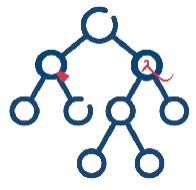
\includegraphics[height=1.0cm]{msca_logo.png}}%
    \end{center}

    \vspace{0.6cm}

    % Main title with Q logos on sides (with clickable links)
    \begin{center}
        \begin{minipage}{0.1\textwidth}
            \centering
            \href{https://quantlet.com}{
\includegraphics[height=1.1cm]{ql_logo.png}}
        \end{minipage}%
        \begin{minipage}{0.78\textwidth}
            \centering
            {\LARGE\bfseries\usebeamercolor[fg]{title}\inserttitle}

            \vspace{0.3cm}

            {\usebeamerfont{subtitle}\usebeamercolor[fg]{title}\insertsubtitle}
        \end{minipage}%
        \begin{minipage}{0.1\textwidth}
            \centering
            \href{https://quantinar.com}{
\includegraphics[height=1.1cm]{qr_logo.png}}
        \end{minipage}
    \end{center}

    \vspace{0.6cm}

    % Authors (left aligned)
    \hspace{0.5cm}{\usebeamerfont{author}\insertauthor}

    \vspace{0.3cm}

    % Institute/Affiliations (left aligned)
    \hspace{0.5cm}\begin{minipage}[t]{0.9\textwidth}
        \raggedright\small\insertinstitute
    \end{minipage}
}

%=============================================================================
% THEOREM ENVIRONMENTS
%=============================================================================
\theoremstyle{definition}
\setbeamertemplate{theorems}[numbered]
\ifdefined\sfmlang
\newtheorem{defn}{Definiție}
\newtheorem{thm}{Teoremă}
\newtheorem{prop}{Propoziție}
\newtheorem{rmk}{Observație}
\else
\newtheorem{defn}{Definition}
\newtheorem{thm}{Theorem}
\newtheorem{prop}{Proposition}
\newtheorem{rmk}{Remark}
\fi

%=============================================================================
% CENTRED MINIPAGE (no extra vertical space)
%=============================================================================
\newenvironment{cminipage}[1]{%
    \par\noindent\hfill\begin{minipage}{#1}\ignorespaces
}{%
    \end{minipage}\hfill\null\par
}

%=============================================================================
% CUSTOM COMMANDS
%=============================================================================
\newcommand{\E}{\mathbb{E}}
\newcommand{\Var}{\text{Var}}
\newcommand{\Cov}{\text{Cov}}
\newcommand{\Corr}{\text{Corr}}
\newcommand{\R}{\mathbb{R}}
\newcommand{\N}{\mathbb{N}}
\newcommand{\Z}{\mathbb{Z}}
\newcommand{\B}{\mathbf{B}}
\newcommand{\imark}{\textcolor{MainBlue}{\textbullet}}
\newcommand{\RMSE}{\text{RMSE}}
\newcommand{\MAE}{\text{MAE}}
\newcommand{\MAPE}{\text{MAPE}}

 se definește
%   \newcommand{\coursename}{Statistics of Financial Markets}      (EN)
%   \newcommand{\coursename}{Statistica piețelor financiare}       (RO)  și  \def\sfmlang{ro}
% Fișierele .tex se află în EN/Courses, EN/Seminars, RO/Cursuri, RO/Seminarii (două niveluri sub rădăcină).
% Deck-urile sînt generate de latex/build_chapterN.py / build_seminarN.py (vezi latex/sfm_build.py).

\documentclass[9pt, aspectratio=169, t]{beamer}
\providecommand{\coursename}{Statistics of Financial Markets}

% Ensure content fits on slides
\setbeamersize{text margin left=8mm, text margin right=8mm}

%=============================================================================
% THEME AND STYLE CONFIGURATION
%=============================================================================
\usetheme{default}
% Using default theme for clean header/footer control

% Color Palette (matching Redispatch PDF)
\definecolor{MainBlue}{RGB}{26, 58, 110}
\definecolor{AccentBlue}{RGB}{26, 58, 110}
\definecolor{IDAred}{RGB}{205, 0, 0}
\definecolor{DarkGray}{RGB}{51, 51, 51}
\definecolor{MediumGray}{RGB}{128, 128, 128}
\definecolor{LightGray}{RGB}{248, 248, 248}
\definecolor{VeryLightGray}{RGB}{235, 235, 235}
\definecolor{KeynoteGray}{RGB}{218, 218, 218}
\definecolor{SectionGray}{RGB}{120, 120, 120}
\definecolor{FooterGray}{RGB}{100, 100, 100}
\definecolor{Crimson}{RGB}{220, 53, 69}
\definecolor{Forest}{RGB}{46, 125, 50}
\definecolor{Amber}{RGB}{181, 133, 63}
\definecolor{Orange}{RGB}{230, 126, 34}
\definecolor{Purple}{RGB}{142, 68, 173}

% Gradient background (exact Keynote 315° gradient: white to RGB 218,218,218)
\setbeamertemplate{background}{%
    \begin{tikzpicture}[remember picture, overlay]
        \shade[shading=axis, shading angle=315,
        top color=white, bottom color=KeynoteGray]
        (current page.south west) rectangle (current page.north east);
    \end{tikzpicture}%
}
% Fallback solid color for compatibility
\setbeamercolor{background canvas}{bg=}

\setbeamercolor{palette primary}{bg=MainBlue, fg=white}
\setbeamercolor{palette secondary}{bg=MainBlue!85, fg=white}
\setbeamercolor{palette tertiary}{bg=MainBlue!70, fg=white}
\setbeamercolor{structure}{fg=MainBlue}
\setbeamercolor{title}{fg=IDAred}
\setbeamercolor{frametitle}{fg=IDAred, bg=}
\setbeamercolor{block title}{bg=MainBlue, fg=white}
\setbeamercolor{block body}{bg=VeryLightGray, fg=DarkGray}
\setbeamercolor{block title alerted}{bg=Crimson, fg=white}
\setbeamercolor{block body alerted}{bg=Crimson!8, fg=DarkGray}
\setbeamercolor{block title example}{bg=Forest, fg=white}
\setbeamercolor{block body example}{bg=Forest!8, fg=DarkGray}
\setbeamercolor{item}{fg=MainBlue}

% Footer colors (override Madrid theme blue)
\setbeamercolor{author in head/foot}{fg=FooterGray, bg=}
\setbeamercolor{title in head/foot}{fg=FooterGray, bg=}
\setbeamercolor{date in head/foot}{fg=FooterGray, bg=}
\setbeamercolor{section in head/foot}{fg=FooterGray, bg=}
\setbeamercolor{subsection in head/foot}{fg=FooterGray, bg=}

% Bullet styles (apply everywhere including blocks)
\setbeamertemplate{itemize item}{\color{MainBlue}$\boxdot$}
\setbeamertemplate{itemize subitem}{\color{MainBlue}$\blacktriangleright$}
\setbeamertemplate{itemize subsubitem}{\color{MainBlue}\tiny$\bullet$}
\setbeamertemplate{itemize/enumerate body begin}{\normalsize}
\setbeamertemplate{itemize/enumerate subbody begin}{\normalsize}

% Item spacing - compact style
\setlength{\leftmargini}{10pt}       % Level 1: minimal indent
\setlength{\leftmarginii}{10pt}      % Level 2: minimal additional indent
% Compact list spacing (zero extra space before/after lists in blocks)
\makeatletter
\def\@listi{\leftmargin\leftmargini \topsep 0pt \parsep 0pt \itemsep 0pt}
\def\@listii{\leftmargin\leftmarginii \topsep 0pt \parsep 0pt \itemsep 0pt}
\makeatother

\setbeamertemplate{navigation symbols}{}

%=============================================================================
% CUSTOM HEADLINE
%=============================================================================
\setbeamertemplate{headline}{%
    \vskip10pt%
    \hbox to \paperwidth{%
        \hskip0.5cm%
        {\small\color{FooterGray}\renewcommand{\hyperlink}[2]{##2}\insertsectionhead}%
        \hfill%
        \textcolor{FooterGray}{\small\insertframenumber}%
        \hskip0.5cm%
    }%
    \vskip4pt%
    {\color{FooterGray}\hrule height 0.4pt}%
}

%=============================================================================
% CUSTOM FOOTER
%=============================================================================
\usepackage{fontawesome5}

\setbeamertemplate{footline}{%
    {\color{FooterGray}\hrule height 0.4pt}%
    \vskip4pt%
    \hbox to \paperwidth{%
        \hskip0.5cm%
        \textcolor{FooterGray}{\small\coursename}%
        \hfill%
        \raisebox{-0.1em}{%
            \begin{tikzpicture}[x=0.08em, y=0.08em, line width=0.4pt]
                \draw[FooterGray] (0,3) -- (1,4) -- (2,3.5) -- (3,5) -- (4,4) -- (5,6) -- (6,5.5) -- (7,4) -- (8,5) -- (9,7) -- (10,6) -- (11,5) -- (12,6.5) -- (13,8) -- (14,7) -- (15,6) -- (16,7.5) -- (17,9) -- (18,8) -- (19,7) -- (20,8.5) -- (21,10) -- (22,9) -- (23,8) -- (24,9.5);
            \end{tikzpicture}%
        }%
        \hskip0.5cm%
    }%
    \vskip6pt%
}

%=============================================================================
% PACKAGES
%=============================================================================
\usepackage[utf8]{inputenc}
\DeclareUnicodeCharacter{03B1}{\ensuremath{\alpha}}
\usepackage[T1]{fontenc}
\usepackage{amsmath, amssymb, amsthm}
\usepackage{mathtools}
\usepackage{bm}
\usepackage{tikz}
\usetikzlibrary{arrows.meta, positioning, shapes, calc, decorations.pathreplacing, shadings}
\usepackage{booktabs}
\usepackage{multirow}
\usepackage{array}
\usepackage{graphicx}
\usepackage{hyperref}
\usepackage{colortbl}
\usepackage{listings}
\lstset{language=Python, basicstyle=\ttfamily\scriptsize, keywordstyle=\color{MainBlue}\bfseries,
  commentstyle=\color{Forest}, stringstyle=\color{Crimson}, breaklines=true,
  frame=none, backgroundcolor=\color{VeryLightGray}, xleftmargin=2mm}
\hypersetup{colorlinks=true, linkcolor=MainBlue, urlcolor=MainBlue}
\graphicspath{{../../logos/}{../../charts/}{../../photos/}}
\usepackage{xcolor}
\hfuzz=2pt  % Suppress tiny overfull warnings (<2pt)
\vfuzz=2pt  % Suppress tiny vertical overfull warnings (<2pt)

%=============================================================================
% QUANTLET COMMANDS
%   \quantlet{<displayed name>}{<url>}       (generic, compatible with the older SFM decks)
%   \sfmquantlet{Ch_05}{SFM_ch5_garch}       -> https://github.com/danpele/SFM/tree/main/Quantlets/Ch_05/SFM_ch5_garch
%   \qlurl{<folder>} is defined per chapter by the generator (Quantlets/Ch_NN/<folder>)
%=============================================================================
\newcommand{\sfmrepo}{https://github.com/danpele/SFM}
\newcommand{\sfmqlbase}{https://github.com/danpele/SFM/tree/main/Quantlets}
\newcommand{\quantlet}[2]{%
    \hfill\href{#2}{%
        \raisebox{-0.15em}{
\includegraphics[height=0.7em]{ql_logo.png}}%
        \textcolor{MainBlue}{\tiny\ #1}%
    }%
}
\newcommand{\sfmquantlet}[2]{\quantlet{\detokenize{#2}}{\sfmqlbase/#1/#2}}

%=============================================================================
% NOTEBOOKS (Google Colab)
%   \colaburl{notebooks/EN/chapter5_seminar_notebook.ipynb} -> the Colab link of a file in the SFM repo
%   \nb: the chapter notebook (each seminar deck redefines it with \renewcommand)
%=============================================================================
\newcommand{\colaburl}[1]{https://colab.research.google.com/github/danpele/SFM/blob/main/#1}
\newcommand{\nb}{https://colab.research.google.com/github/danpele/SFM/tree/main/notebooks/EN}
\newcommand{\nbname}{notebooks/EN}

%=============================================================================
% SLIDE HELPERS (used by the generators; the same as in MFM)
%=============================================================================
% local font size for list bodies (the preamble forces \normalsize)
\newcommand{\itemsize}[1]{\setbeamertemplate{itemize/enumerate body begin}{#1}\setbeamertemplate{itemize/enumerate subbody begin}{#1}}
\newcommand{\intitle}[1]{{\hypersetup{urlcolor=white}#1}}   % white links inside coloured title bars
\newcommand{\imgcap}[1]{{\scriptsize #1}\\[0.5mm]}          % caption under a photo
\newcommand{\imgcredit}[2]{{\tiny\color{FooterGray}\href{#1}{#2}}}   % image credit: source URL, author/licence
\newcommand{\aiprompt}[1]{{\ttfamily\color{MainBlue}#1}}     % a prompt to an AI assistant

%=============================================================================
% SEMINARS: student version by default; the instructor wrapper *_solutions.tex sets \solutionstrue
%=============================================================================
\makeatletter\@ifundefined{ifsolutions}{\expandafter\newif\csname ifsolutions\endcsname}{}\makeatother
\newcommand{\solonly}[1]{\ifsolutions #1\fi}
\newcommand{\propsub}{\ifsolutions\else\framesubtitle{\ifdefined\sfmlang Rezolvarea se discută la seminar\else Solution discussed in class\fi}\fi}

%=============================================================================
% APPENDIX AND CHAPTER LINKS (latex/appendix_links.py writes the calls; it also re-declares these
% macros before \begin{document}, so the decks compile with or without this preamble block)
%=============================================================================
\providecommand{\sfmapplink}[3]{\hypertarget{#2}{}\hyperlink{#1}{\beamergotobutton{#3}}}
\providecommand{\sfmappback}[2]{\begin{tikzpicture}[remember picture,overlay]\node[anchor=south east] at ([xshift=-3mm,yshift=7mm]current page.south east){\hyperlink{#1}{\beamerreturnbutton{#2}}};\end{tikzpicture}}
\providecommand{\sfmchlink}[2]{\href{#1}{#2}}
\providecommand{\sfmchlinkt}[2]{\href{#1}{\usebeamercolor[fg]{frametitle}#2}}

%=============================================================================
% QUANTINAR COMMAND: link către un curs Quantinar (subiecte avansate)
%=============================================================================
\newcommand{\quantinar}[2]{%
    \href{#2}{%
        \raisebox{-0.15em}{
\includegraphics[height=0.8em]{qr_logo.png}}%
        \textcolor{MainBlue}{\scriptsize\ #1}%
    }%
}

%=============================================================================
% CUSTOM TITLE PAGE
%=============================================================================
\defbeamertemplate*{title page}{hybrid}[1][]
{
    \vspace{0.2cm}
    % Logos row - top header (with clickable links)
    \begin{center}
        \href{https://www.ase.ro}{
\includegraphics[height=1.0cm]{ase_logo.png}}\hspace{0.3cm}%
        \href{https://theida.net}{
\includegraphics[height=1.0cm]{ida_logo.png}}\hspace{0.3cm}%
        \href{https://blockchain-research-center.com}{
\includegraphics[height=1.0cm]{brc_logo.png}}\hspace{0.3cm}%
        \href{https://www.ai4efin.ase.ro}{
\includegraphics[height=1.0cm]{ai4efin_logo.png}}\hspace{0.3cm}%
        \href{https://ipe.ro/new}{
\includegraphics[height=1.0cm]{acad_logo.png}}\hspace{0.3cm}%
        \href{https://www.digital-finance-msca.com}{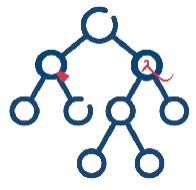
\includegraphics[height=1.0cm]{msca_logo.png}}%
    \end{center}

    \vspace{0.6cm}

    % Main title with Q logos on sides (with clickable links)
    \begin{center}
        \begin{minipage}{0.1\textwidth}
            \centering
            \href{https://quantlet.com}{
\includegraphics[height=1.1cm]{ql_logo.png}}
        \end{minipage}%
        \begin{minipage}{0.78\textwidth}
            \centering
            {\LARGE\bfseries\usebeamercolor[fg]{title}\inserttitle}

            \vspace{0.3cm}

            {\usebeamerfont{subtitle}\usebeamercolor[fg]{title}\insertsubtitle}
        \end{minipage}%
        \begin{minipage}{0.1\textwidth}
            \centering
            \href{https://quantinar.com}{
\includegraphics[height=1.1cm]{qr_logo.png}}
        \end{minipage}
    \end{center}

    \vspace{0.6cm}

    % Authors (left aligned)
    \hspace{0.5cm}{\usebeamerfont{author}\insertauthor}

    \vspace{0.3cm}

    % Institute/Affiliations (left aligned)
    \hspace{0.5cm}\begin{minipage}[t]{0.9\textwidth}
        \raggedright\small\insertinstitute
    \end{minipage}
}

%=============================================================================
% THEOREM ENVIRONMENTS
%=============================================================================
\theoremstyle{definition}
\setbeamertemplate{theorems}[numbered]
\ifdefined\sfmlang
\newtheorem{defn}{Definiție}
\newtheorem{thm}{Teoremă}
\newtheorem{prop}{Propoziție}
\newtheorem{rmk}{Observație}
\else
\newtheorem{defn}{Definition}
\newtheorem{thm}{Theorem}
\newtheorem{prop}{Proposition}
\newtheorem{rmk}{Remark}
\fi

%=============================================================================
% CENTRED MINIPAGE (no extra vertical space)
%=============================================================================
\newenvironment{cminipage}[1]{%
    \par\noindent\hfill\begin{minipage}{#1}\ignorespaces
}{%
    \end{minipage}\hfill\null\par
}

%=============================================================================
% CUSTOM COMMANDS
%=============================================================================
\newcommand{\E}{\mathbb{E}}
\newcommand{\Var}{\text{Var}}
\newcommand{\Cov}{\text{Cov}}
\newcommand{\Corr}{\text{Corr}}
\newcommand{\R}{\mathbb{R}}
\newcommand{\N}{\mathbb{N}}
\newcommand{\Z}{\mathbb{Z}}
\newcommand{\B}{\mathbf{B}}
\newcommand{\imark}{\textcolor{MainBlue}{\textbullet}}
\newcommand{\RMSE}{\text{RMSE}}
\newcommand{\MAE}{\text{MAE}}
\newcommand{\MAPE}{\text{MAPE}}

 se definește
%   \newcommand{\coursename}{Statistics of Financial Markets}      (EN)
%   \newcommand{\coursename}{Statistica piețelor financiare}       (RO)  și  \def\sfmlang{ro}
% Fișierele .tex se află în EN/Courses, EN/Seminars, RO/Cursuri, RO/Seminarii (două niveluri sub rădăcină).
% Deck-urile sînt generate de latex/build_chapterN.py / build_seminarN.py (vezi latex/sfm_build.py).

\documentclass[9pt, aspectratio=169, t]{beamer}
\providecommand{\coursename}{Statistics of Financial Markets}

% Ensure content fits on slides
\setbeamersize{text margin left=8mm, text margin right=8mm}

%=============================================================================
% THEME AND STYLE CONFIGURATION
%=============================================================================
\usetheme{default}
% Using default theme for clean header/footer control

% Color Palette (matching Redispatch PDF)
\definecolor{MainBlue}{RGB}{26, 58, 110}
\definecolor{AccentBlue}{RGB}{26, 58, 110}
\definecolor{IDAred}{RGB}{205, 0, 0}
\definecolor{DarkGray}{RGB}{51, 51, 51}
\definecolor{MediumGray}{RGB}{128, 128, 128}
\definecolor{LightGray}{RGB}{248, 248, 248}
\definecolor{VeryLightGray}{RGB}{235, 235, 235}
\definecolor{KeynoteGray}{RGB}{218, 218, 218}
\definecolor{SectionGray}{RGB}{120, 120, 120}
\definecolor{FooterGray}{RGB}{100, 100, 100}
\definecolor{Crimson}{RGB}{220, 53, 69}
\definecolor{Forest}{RGB}{46, 125, 50}
\definecolor{Amber}{RGB}{181, 133, 63}
\definecolor{Orange}{RGB}{230, 126, 34}
\definecolor{Purple}{RGB}{142, 68, 173}

% Gradient background (exact Keynote 315° gradient: white to RGB 218,218,218)
\setbeamertemplate{background}{%
    \begin{tikzpicture}[remember picture, overlay]
        \shade[shading=axis, shading angle=315,
        top color=white, bottom color=KeynoteGray]
        (current page.south west) rectangle (current page.north east);
    \end{tikzpicture}%
}
% Fallback solid color for compatibility
\setbeamercolor{background canvas}{bg=}

\setbeamercolor{palette primary}{bg=MainBlue, fg=white}
\setbeamercolor{palette secondary}{bg=MainBlue!85, fg=white}
\setbeamercolor{palette tertiary}{bg=MainBlue!70, fg=white}
\setbeamercolor{structure}{fg=MainBlue}
\setbeamercolor{title}{fg=IDAred}
\setbeamercolor{frametitle}{fg=IDAred, bg=}
\setbeamercolor{block title}{bg=MainBlue, fg=white}
\setbeamercolor{block body}{bg=VeryLightGray, fg=DarkGray}
\setbeamercolor{block title alerted}{bg=Crimson, fg=white}
\setbeamercolor{block body alerted}{bg=Crimson!8, fg=DarkGray}
\setbeamercolor{block title example}{bg=Forest, fg=white}
\setbeamercolor{block body example}{bg=Forest!8, fg=DarkGray}
\setbeamercolor{item}{fg=MainBlue}

% Footer colors (override Madrid theme blue)
\setbeamercolor{author in head/foot}{fg=FooterGray, bg=}
\setbeamercolor{title in head/foot}{fg=FooterGray, bg=}
\setbeamercolor{date in head/foot}{fg=FooterGray, bg=}
\setbeamercolor{section in head/foot}{fg=FooterGray, bg=}
\setbeamercolor{subsection in head/foot}{fg=FooterGray, bg=}

% Bullet styles (apply everywhere including blocks)
\setbeamertemplate{itemize item}{\color{MainBlue}$\boxdot$}
\setbeamertemplate{itemize subitem}{\color{MainBlue}$\blacktriangleright$}
\setbeamertemplate{itemize subsubitem}{\color{MainBlue}\tiny$\bullet$}
\setbeamertemplate{itemize/enumerate body begin}{\normalsize}
\setbeamertemplate{itemize/enumerate subbody begin}{\normalsize}

% Item spacing - compact style
\setlength{\leftmargini}{10pt}       % Level 1: minimal indent
\setlength{\leftmarginii}{10pt}      % Level 2: minimal additional indent
% Compact list spacing (zero extra space before/after lists in blocks)
\makeatletter
\def\@listi{\leftmargin\leftmargini \topsep 0pt \parsep 0pt \itemsep 0pt}
\def\@listii{\leftmargin\leftmarginii \topsep 0pt \parsep 0pt \itemsep 0pt}
\makeatother

\setbeamertemplate{navigation symbols}{}

%=============================================================================
% CUSTOM HEADLINE
%=============================================================================
\setbeamertemplate{headline}{%
    \vskip10pt%
    \hbox to \paperwidth{%
        \hskip0.5cm%
        {\small\color{FooterGray}\renewcommand{\hyperlink}[2]{##2}\insertsectionhead}%
        \hfill%
        \textcolor{FooterGray}{\small\insertframenumber}%
        \hskip0.5cm%
    }%
    \vskip4pt%
    {\color{FooterGray}\hrule height 0.4pt}%
}

%=============================================================================
% CUSTOM FOOTER
%=============================================================================
\usepackage{fontawesome5}

\setbeamertemplate{footline}{%
    {\color{FooterGray}\hrule height 0.4pt}%
    \vskip4pt%
    \hbox to \paperwidth{%
        \hskip0.5cm%
        \textcolor{FooterGray}{\small\coursename}%
        \hfill%
        \raisebox{-0.1em}{%
            \begin{tikzpicture}[x=0.08em, y=0.08em, line width=0.4pt]
                \draw[FooterGray] (0,3) -- (1,4) -- (2,3.5) -- (3,5) -- (4,4) -- (5,6) -- (6,5.5) -- (7,4) -- (8,5) -- (9,7) -- (10,6) -- (11,5) -- (12,6.5) -- (13,8) -- (14,7) -- (15,6) -- (16,7.5) -- (17,9) -- (18,8) -- (19,7) -- (20,8.5) -- (21,10) -- (22,9) -- (23,8) -- (24,9.5);
            \end{tikzpicture}%
        }%
        \hskip0.5cm%
    }%
    \vskip6pt%
}

%=============================================================================
% PACKAGES
%=============================================================================
\usepackage[utf8]{inputenc}
\DeclareUnicodeCharacter{03B1}{\ensuremath{\alpha}}
\usepackage[T1]{fontenc}
\usepackage{amsmath, amssymb, amsthm}
\usepackage{mathtools}
\usepackage{bm}
\usepackage{tikz}
\usetikzlibrary{arrows.meta, positioning, shapes, calc, decorations.pathreplacing, shadings}
\usepackage{booktabs}
\usepackage{multirow}
\usepackage{array}
\usepackage{graphicx}
\usepackage{hyperref}
\usepackage{colortbl}
\usepackage{listings}
\lstset{language=Python, basicstyle=\ttfamily\scriptsize, keywordstyle=\color{MainBlue}\bfseries,
  commentstyle=\color{Forest}, stringstyle=\color{Crimson}, breaklines=true,
  frame=none, backgroundcolor=\color{VeryLightGray}, xleftmargin=2mm}
\hypersetup{colorlinks=true, linkcolor=MainBlue, urlcolor=MainBlue}
\graphicspath{{../../logos/}{../../charts/}{../../photos/}}
\usepackage{xcolor}
\hfuzz=2pt  % Suppress tiny overfull warnings (<2pt)
\vfuzz=2pt  % Suppress tiny vertical overfull warnings (<2pt)

%=============================================================================
% QUANTLET COMMANDS
%   \quantlet{<displayed name>}{<url>}       (generic, compatible with the older SFM decks)
%   \sfmquantlet{Ch_05}{SFM_ch5_garch}       -> https://github.com/danpele/SFM/tree/main/Quantlets/Ch_05/SFM_ch5_garch
%   \qlurl{<folder>} is defined per chapter by the generator (Quantlets/Ch_NN/<folder>)
%=============================================================================
\newcommand{\sfmrepo}{https://github.com/danpele/SFM}
\newcommand{\sfmqlbase}{https://github.com/danpele/SFM/tree/main/Quantlets}
\newcommand{\quantlet}[2]{%
    \hfill\href{#2}{%
        \raisebox{-0.15em}{
\includegraphics[height=0.7em]{ql_logo.png}}%
        \textcolor{MainBlue}{\tiny\ #1}%
    }%
}
\newcommand{\sfmquantlet}[2]{\quantlet{\detokenize{#2}}{\sfmqlbase/#1/#2}}

%=============================================================================
% NOTEBOOKS (Google Colab)
%   \colaburl{notebooks/EN/chapter5_seminar_notebook.ipynb} -> the Colab link of a file in the SFM repo
%   \nb: the chapter notebook (each seminar deck redefines it with \renewcommand)
%=============================================================================
\newcommand{\colaburl}[1]{https://colab.research.google.com/github/danpele/SFM/blob/main/#1}
\newcommand{\nb}{https://colab.research.google.com/github/danpele/SFM/tree/main/notebooks/EN}
\newcommand{\nbname}{notebooks/EN}

%=============================================================================
% SLIDE HELPERS (used by the generators; the same as in MFM)
%=============================================================================
% local font size for list bodies (the preamble forces \normalsize)
\newcommand{\itemsize}[1]{\setbeamertemplate{itemize/enumerate body begin}{#1}\setbeamertemplate{itemize/enumerate subbody begin}{#1}}
\newcommand{\intitle}[1]{{\hypersetup{urlcolor=white}#1}}   % white links inside coloured title bars
\newcommand{\imgcap}[1]{{\scriptsize #1}\\[0.5mm]}          % caption under a photo
\newcommand{\imgcredit}[2]{{\tiny\color{FooterGray}\href{#1}{#2}}}   % image credit: source URL, author/licence
\newcommand{\aiprompt}[1]{{\ttfamily\color{MainBlue}#1}}     % a prompt to an AI assistant

%=============================================================================
% SEMINARS: student version by default; the instructor wrapper *_solutions.tex sets \solutionstrue
%=============================================================================
\makeatletter\@ifundefined{ifsolutions}{\expandafter\newif\csname ifsolutions\endcsname}{}\makeatother
\newcommand{\solonly}[1]{\ifsolutions #1\fi}
\newcommand{\propsub}{\ifsolutions\else\framesubtitle{\ifdefined\sfmlang Rezolvarea se discută la seminar\else Solution discussed in class\fi}\fi}

%=============================================================================
% APPENDIX AND CHAPTER LINKS (latex/appendix_links.py writes the calls; it also re-declares these
% macros before \begin{document}, so the decks compile with or without this preamble block)
%=============================================================================
\providecommand{\sfmapplink}[3]{\hypertarget{#2}{}\hyperlink{#1}{\beamergotobutton{#3}}}
\providecommand{\sfmappback}[2]{\begin{tikzpicture}[remember picture,overlay]\node[anchor=south east] at ([xshift=-3mm,yshift=7mm]current page.south east){\hyperlink{#1}{\beamerreturnbutton{#2}}};\end{tikzpicture}}
\providecommand{\sfmchlink}[2]{\href{#1}{#2}}
\providecommand{\sfmchlinkt}[2]{\href{#1}{\usebeamercolor[fg]{frametitle}#2}}

%=============================================================================
% QUANTINAR COMMAND: link către un curs Quantinar (subiecte avansate)
%=============================================================================
\newcommand{\quantinar}[2]{%
    \href{#2}{%
        \raisebox{-0.15em}{
\includegraphics[height=0.8em]{qr_logo.png}}%
        \textcolor{MainBlue}{\scriptsize\ #1}%
    }%
}

%=============================================================================
% CUSTOM TITLE PAGE
%=============================================================================
\defbeamertemplate*{title page}{hybrid}[1][]
{
    \vspace{0.2cm}
    % Logos row - top header (with clickable links)
    \begin{center}
        \href{https://www.ase.ro}{
\includegraphics[height=1.0cm]{ase_logo.png}}\hspace{0.3cm}%
        \href{https://theida.net}{
\includegraphics[height=1.0cm]{ida_logo.png}}\hspace{0.3cm}%
        \href{https://blockchain-research-center.com}{
\includegraphics[height=1.0cm]{brc_logo.png}}\hspace{0.3cm}%
        \href{https://www.ai4efin.ase.ro}{
\includegraphics[height=1.0cm]{ai4efin_logo.png}}\hspace{0.3cm}%
        \href{https://ipe.ro/new}{
\includegraphics[height=1.0cm]{acad_logo.png}}\hspace{0.3cm}%
        \href{https://www.digital-finance-msca.com}{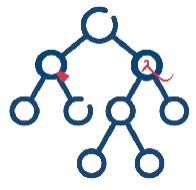
\includegraphics[height=1.0cm]{msca_logo.png}}%
    \end{center}

    \vspace{0.6cm}

    % Main title with Q logos on sides (with clickable links)
    \begin{center}
        \begin{minipage}{0.1\textwidth}
            \centering
            \href{https://quantlet.com}{
\includegraphics[height=1.1cm]{ql_logo.png}}
        \end{minipage}%
        \begin{minipage}{0.78\textwidth}
            \centering
            {\LARGE\bfseries\usebeamercolor[fg]{title}\inserttitle}

            \vspace{0.3cm}

            {\usebeamerfont{subtitle}\usebeamercolor[fg]{title}\insertsubtitle}
        \end{minipage}%
        \begin{minipage}{0.1\textwidth}
            \centering
            \href{https://quantinar.com}{
\includegraphics[height=1.1cm]{qr_logo.png}}
        \end{minipage}
    \end{center}

    \vspace{0.6cm}

    % Authors (left aligned)
    \hspace{0.5cm}{\usebeamerfont{author}\insertauthor}

    \vspace{0.3cm}

    % Institute/Affiliations (left aligned)
    \hspace{0.5cm}\begin{minipage}[t]{0.9\textwidth}
        \raggedright\small\insertinstitute
    \end{minipage}
}

%=============================================================================
% THEOREM ENVIRONMENTS
%=============================================================================
\theoremstyle{definition}
\setbeamertemplate{theorems}[numbered]
\ifdefined\sfmlang
\newtheorem{defn}{Definiție}
\newtheorem{thm}{Teoremă}
\newtheorem{prop}{Propoziție}
\newtheorem{rmk}{Observație}
\else
\newtheorem{defn}{Definition}
\newtheorem{thm}{Theorem}
\newtheorem{prop}{Proposition}
\newtheorem{rmk}{Remark}
\fi

%=============================================================================
% CENTRED MINIPAGE (no extra vertical space)
%=============================================================================
\newenvironment{cminipage}[1]{%
    \par\noindent\hfill\begin{minipage}{#1}\ignorespaces
}{%
    \end{minipage}\hfill\null\par
}

%=============================================================================
% CUSTOM COMMANDS
%=============================================================================
\newcommand{\E}{\mathbb{E}}
\newcommand{\Var}{\text{Var}}
\newcommand{\Cov}{\text{Cov}}
\newcommand{\Corr}{\text{Corr}}
\newcommand{\R}{\mathbb{R}}
\newcommand{\N}{\mathbb{N}}
\newcommand{\Z}{\mathbb{Z}}
\newcommand{\B}{\mathbf{B}}
\newcommand{\imark}{\textcolor{MainBlue}{\textbullet}}
\newcommand{\RMSE}{\text{RMSE}}
\newcommand{\MAE}{\text{MAE}}
\newcommand{\MAPE}{\text{MAPE}}



\newcommand{\qlurl}[1]{https://github.com/danpele/SFM/tree/main/Quantlets/Ch_14/#1}
\renewcommand{\nb}{\colaburl{notebooks/EN/chapter14_seminar_notebook.ipynb}}
\renewcommand{\nbname}{chapter14\_seminar\_notebook.ipynb}
% left column: full width in the student version, narrower next to the solution
\newcommand{\taskw}{\ifsolutions 0.47\textwidth\else 0.96\textwidth\fi}
\newcommand{\solw}{\ifsolutions 0.49\textwidth\else 0pt\fi}

% Clickable citations (DOIs verified via Crossref)

\newcommand{\refNakamoto}{\href{https://bitcoin.org/bitcoin.pdf}{Nakamoto (2008)}}
\newcommand{\refButerin}{\href{https://ethereum.org/en/whitepaper/}{Buterin (2014)}}
\newcommand{\refMerge}{\href{https://ethereum.org/en/roadmap/merge/}{ethereum.org: The Merge}}
\newcommand{\refLT}{\href{https://doi.org/10.1093/rfs/hhaa113}{Liu \& Tsyvinski (2021)}}
\newcommand{\refLTW}{\href{https://doi.org/10.1111/jofi.13119}{Liu, Tsyvinski \& Wu (2022)}}
\newcommand{\refGS}{\href{https://doi.org/10.1111/jofi.12903}{Griffin \& Shams (2020)}}
\newcommand{\refMS}{\href{https://doi.org/10.1016/j.jfineco.2019.07.001}{Makarov \& Schoar (2020)}}
\newcommand{\refGorton}{\href{https://doi.org/10.3386/w30796}{Gorton et al.\ (2022)}}
\newcommand{\refGZ}{\href{https://doi.org/10.2139/ssrn.3888752}{Gorton \& Zhang (2021)}}
\newcommand{\refLVN}{\href{https://doi.org/10.1016/j.jimonfin.2022.102777}{Lyons \& Viswanath-Natraj (2023)}}
\newcommand{\refLMS}{\href{https://doi.org/10.3386/w31160}{Liu, Makarov \& Schoar (2023)}}
\newcommand{\refMZZ}{\href{https://doi.org/10.3386/w33882}{Ma, Zeng \& Zhang (2025)}}
\newcommand{\refUrquhart}{\href{https://doi.org/10.1016/j.econlet.2016.09.019}{Urquhart (2016)}}
\newcommand{\refNC}{\href{https://doi.org/10.1016/j.econlet.2016.10.033}{Nadarajah \& Chu (2017)}}
\newcommand{\refTL}{\href{https://doi.org/10.1016/j.frl.2019.101382}{Tran \& Leirvik (2020)}}
\newcommand{\refCF}{\href{https://doi.org/10.1016/j.econlet.2015.02.029}{Cheah \& Fry (2015)}}
\newcommand{\refKatsiampa}{\href{https://doi.org/10.1016/j.econlet.2017.06.023}{Katsiampa (2017)}}
\newcommand{\refBL}{\href{https://doi.org/10.1111/j.1540-6288.2010.00244.x}{Baur \& Lucey (2010)}}
\newcommand{\refBHL}{\href{https://doi.org/10.1016/j.intfin.2017.12.004}{Baur, Hong \& Lee (2018)}}
\newcommand{\refCP}{\href{https://doi.org/10.1016/j.frl.2018.11.012}{Caporale \& Plastun (2019)}}
\newcommand{\refGHMO}{\href{https://doi.org/10.1016/j.jmoneco.2017.12.004}{Gandal et al.\ (2018)}}
\newcommand{\refHill}{\href{https://doi.org/10.1214/aos/1176343247}{Hill (1975)}}
\newcommand{\refBoll}{\href{https://doi.org/10.1016/0304-4076(86)90063-1}{Bollerslev (1986)}}
\newcommand{\refLM}{\href{https://doi.org/10.1093/rfs/1.1.41}{Lo \& MacKinlay (1988)}}
\newcommand{\refFama}{\href{https://doi.org/10.2307/2325486}{Fama (1970)}}
\newcommand{\refJLS}{\href{https://doi.org/10.1142/S0219024900000115}{Johansen, Ledoit \& Sornette (2000)}}
\newcommand{\refTH}{\href{https://doi.org/10.1016/j.jempfin.2018.08.004}{Trimborn \& Härdle (2018)}}
\newcommand{\refHHR}{\href{https://doi.org/10.1093/jjfinec/nbz033}{Härdle, Harvey \& Reule (2020)}}
\newcommand{\refFHH}{\href{https://doi.org/10.1007/978-3-030-13751-9}{Franke, Härdle \& Hafner (2019)}}
\newcommand{\refKupiec}{\href{https://doi.org/10.3905/jod.1995.407942}{Kupiec (1995)}}
\newcommand{\refWang}{\href{https://doi.org/10.1038/s41586-023-06221-2}{Wang et al.\ (2023)}}
\newcommand{\refPeleA}{\href{https://doi.org/10.1080/1351847X.2021.1960403}{Pele et al.\ (2023)}}
\newcommand{\refPeleB}{\href{https://doi.org/10.3390/e21020102}{Pele \& Mazurencu-Marinescu-Pele (2019)}}
\newcommand{\refMiCA}{\href{https://eur-lex.europa.eu/eli/reg/2023/1114/oj}{Regulation (EU) 2023/1114 (MiCA)}}
\newcommand{\refESMA}{\href{https://www.esma.europa.eu/esmas-activities/digital-finance-and-innovation/markets-crypto-assets-regulation-mica}{ESMA: MiCA}}
\newcommand{\refGENIUS}{\href{https://www.govinfo.gov/app/details/PLAW-119publ27}{GENIUS Act, Public Law 119-27}}
\newcommand{\refSEC}{\href{https://www.sec.gov/newsroom/speeches-statements/gensler-statement-spot-bitcoin-011023}{SEC (2024)}}
\newcommand{\refFed}{\href{https://www.federalreserve.gov/newsevents/pressreleases/monetary20230312b.htm}{Treasury, Federal Reserve and FDIC (2023)}}
\newcommand{\refFDIC}{\href{https://www.fdic.gov/news/press-releases/2023/pr23016.html}{FDIC (2023)}}
\newcommand{\refDL}{\href{https://api-docs.defillama.com/}{DefiLlama}}

\title[Statistics of Financial Markets]{Statistics of Financial Markets}
\subtitle{Seminar 14: Crypto assets\ifsolutions\ (instructor version)\fi}
\author[D.T. Pele]{Daniel Traian PELE}
\institute{Bucharest University of Economic Studies\\
IDA Institute Digital Assets\\
Blockchain Research Center\\
AI4EFin Artificial Intelligence for Energy Finance\\
Romanian Academy, Institute for Economic Forecasting\\
MSCA Digital Finance}
\date{}

%=============================================================================
\providecommand{\sfmapplink}[3]{\hypertarget{#2}{}\hyperlink{#1}{\beamergotobutton{#3}}}  % APPLINKS-MACROS
\providecommand{\sfmappback}[2]{\begin{tikzpicture}[remember picture,overlay]\node[anchor=south east] at ([xshift=-3mm,yshift=7mm]current page.south east){\hyperlink{#1}{\beamerreturnbutton{#2}}};\end{tikzpicture}}  % APPLINKS-MACROS
\providecommand{\sfmchlink}[2]{\href{#1}{#2}}  % APPLINKS-MACROS
\providecommand{\sfmchlinkt}[2]{\href{#1}{\usebeamercolor[fg]{frametitle}#2}}  % APPLINKS-MACROS
\begin{document}
%=============================================================================

{
\setbeamertemplate{headline}{}
\setbeamertemplate{footline}{}
\begin{frame}[noframenumbering]
    \titlepage
\end{frame}
}
% BEGIN-ACRONYMS (generat de latex/acronyms.py; nu editati manual)
\begin{frame}{Acronyms used in this material}
\setbeamertemplate{itemize/enumerate body begin}{\tiny}
\begin{columns}[T]
\begin{column}{0.49\textwidth}
\begin{itemize}\setlength{\itemsep}{0pt}
    \item \textbf{AI}: Artificial Intelligence
    \item \textbf{AR}: AutoRegressive (model); in event studies: Abnormal Return
    \item \textbf{CI}: Confidence Interval
    \item \textbf{COVID-19}: COronaVIrus Disease 2019
    \item \textbf{DAI}: Dai (stablecoin of the MakerDAO protocol)
    \item \textbf{EODHD}: EOD Historical Data (market-data provider)
    \item \textbf{ES}: Expected Shortfall
    \item \textbf{ETF}: Exchange-Traded Fund
    \item \textbf{FTX}: FTX Trading Ltd. (crypto exchange, bankrupt in November 2022)
    \item \textbf{GARCH}: Generalised AutoRegressive Conditional Heteroskedasticity
    \item \textbf{HS}: Historical Simulation
    \item \textbf{LR}: Likelihood Ratio
    \item \textbf{LUNA}: Luna (token of the Terra blockchain)
\end{itemize}
\end{column}
\begin{column}{0.49\textwidth}
\begin{itemize}\setlength{\itemsep}{0pt}
    \item \textbf{SVB}: Silicon Valley Bank
    \item \textbf{US}: United States
    \item \textbf{USDC}: USD Coin
    \item \textbf{UST}: TerraUSD
\end{itemize}
\end{column}
\end{columns}
\end{frame}
% END-ACRONYMS

\begin{frame}{Today's Question and Route}
\itemsize{\small}
\begin{itemize}
    \item \textbf{Question}: how risky is a crypto position, and how stable is a ``stable'' coin?
    \begin{itemize}
        \item this seminar comes \textbf{before} Lecture 14: the section ``What You Need for Today'' gives every definition the tasks use
    \end{itemize}
    \item Route
    \begin{itemize}
        \item Part A: annualisation with 365 days, drawdowns, peg deviations in basis points, VaR of a crypto position, on paper
        \item Part B: tails, correlation with equities, the peg of USDC and a backtest of Bitcoin VaR on real data, each with an interpretation question
        \item Part C: an open question for a project and an AI answer to audit
    \end{itemize}
    \item Notebook for today: \href{\nb}{open the seminar notebook in Google Colab}; each task names its notebook section
    \item The seminar is for practice and is not graded; the solutions of [Proposed] tasks are discussed in class
\end{itemize}
\end{frame}

\begin{frame}{Exercise Map}
\itemsize{\footnotesize}
\begin{center}
\scriptsize
\begin{tabular}{>{\raggedright\arraybackslash}p{1.1cm}>{\raggedright\arraybackslash}p{7.5cm}>{\raggedright\arraybackslash}p{1.9cm}>{\raggedright\arraybackslash}p{1.4cm}}
\toprule
\textbf{Task} & \textbf{Question} & \textbf{Type} & \textbf{Model} \\
\midrule
A1, A2 & annualising a crypto series with 365 and with 252 days & Solved, Proposed & A1 \\
A3, A4 & the maximum drawdown of a price path and the gain needed to recover & Solved, Proposed & A3 \\
A5, A6 & peg deviations of USDC and DAI in March 2023, in basis points & Solved, Proposed & A5 \\
A7, A8 & VaR 1\% and ES 2.5\% of a Bitcoin and of an Ethereum position & Solved, Proposed & A7 \\
B1, B2 & moments, annualisation and tail index: Bitcoin and S\&P 500; Ethereum and Solana & Solved, Proposed & B1 \\
B3, B4 & correlation in calm and crisis periods: Bitcoin and S\&P 500; Bitcoin and gold, Ethereum and S\&P 500 & Solved, Proposed & B3 \\
B5, B6 & the peg of USDC; USDT and DAI & Solved, Proposed & B5 \\
B7, B8 & VaR, ES and a backtest: Bitcoin; Ethereum & Solved, Proposed & B7 \\
C1, C2 & did the spot ETFs change Bitcoin? what is wrong in an AI answer? & Proposed & B1, B3 \\
\bottomrule
\end{tabular}
\end{center}
\begin{itemize}
    \item \textbf{[Solved]}: full solution in the slides and in the notebook, a model to follow; \textbf{[Proposed]}: you solve it, following the model
\end{itemize}
\end{frame}

\begin{frame}{Data Used}
\itemsize{\small}
\begin{center}
\footnotesize
\begin{tabular}{llll}
\toprule
\textbf{Series} & \textbf{Source} & \textbf{Price used} & \textbf{Period} \\
\midrule
Bitcoin, Ethereum, Solana & EODHD & close, 7 days a week & 2014/2016/2020--2026 \\
USDT, USDC, DAI & EODHD & close and daily low & 2021--2026 \\
S\&P 500, gold (XAU/USD) & EODHD & close, weekdays & 2014--2026 \\
\bottomrule
\end{tabular}
\end{center}
\begin{itemize}
    \item Daily log returns in \%: $r_t = 100\,(\ln P_t - \ln P_{t-1})$, each series on its own calendar; the last day is 18 September 2026
    \item Two series together: join the prices on common days first, then compute returns
    \item In the notebook: \texttt{returns('btc')}, \texttt{joint\_returns('btc', 'sp500')}, \texttt{describe(k)}, \texttt{peg\_stats('usdc')}; no account or key is needed
\end{itemize}
\end{frame}


%=============================================================================
\section{What You Need for Today}
%=============================================================================

\begin{frame}{What You Need for Today (1/4): Crypto Assets and Annualisation}
\itemsize{\small}
\begin{itemize}
    \item \textbf{Crypto asset}: a digital asset whose ownership is recorded on a \textbf{blockchain}, a public chain of blocks of transactions
    \begin{itemize}
        \item Bitcoin (2009): fixed supply of 21 million coins; Ethereum (2015): runs programs (smart contracts)
        \item traded on \textbf{exchanges} (trading platforms) 24 hours a day, 7 days a week
    \end{itemize}
    \item \textbf{Annualisation} with $m$ observations a year (i.i.d.\ returns): mean $m\,\bar r$, volatility $\sqrt{m}\,s$
    \begin{itemize}
        \item crypto: $m = 365$, $\sqrt{365} = 19.105$; equities: $m = 252$, $\sqrt{252} = 15.875$
        \item \textbf{Sharpe ratio} (risk-free rate 0): annual mean / annual volatility $= \sqrt{m}\,\bar r/s$
    \end{itemize}
    \item Hill tail index (\sfmchlink{https://danpele.github.io/SFM/EN/Courses/chapter5_heavy_tails_evt.pdf}{Chapter 5}): $\hat\alpha = [\frac1k\sum_{i \le k}\ln(X_{(i)}/X_{(k+1)})]^{-1}$ on the $k$ largest losses; 95\% CI $\hat\alpha(1 \pm 1.96/\sqrt{k})$; smaller $\alpha$, heavier tail
\end{itemize}
\end{frame}

\begin{frame}{What You Need for Today (2/4): Drawdown and Correlation}
\itemsize{\small}
\begin{itemize}
    \item \textbf{Drawdown}: $D_t = P_t/M_t - 1$, $M_t = \max_{s \le t} P_s$ the running maximum (the last record high)
    \begin{itemize}
        \item \textbf{maximum drawdown} $= \min_t D_t$; to recover from a loss $d$, the price must rise by $d/(1 - d)$
    \end{itemize}
    \item \textbf{Correlation} of two series with different calendars: join the prices on common days, then compute log returns
    \begin{itemize}
        \item Fisher $z$: $z = \tanh^{-1}(\hat\rho)$ is approximately $N(\tanh^{-1}\rho, 1/(n - 3))$; 95\% CI: $\tanh(z \pm 1.96/\sqrt{n - 3})$
        \item two independent periods: $(z_2 - z_1)/\sqrt{1/(n_1 - 3) + 1/(n_2 - 3)} \sim N(0, 1)$ if $\rho_1 = \rho_2$
    \end{itemize}
    \item \textbf{Safe haven} \refBL: an asset that does not fall (or rises) when the stock market crashes
\end{itemize}
\end{frame}

\begin{frame}{What You Need for Today (3/4): Stablecoins and Basis Points}
\itemsize{\small}
\begin{itemize}
    \item \textbf{Stablecoin}: a crypto asset designed to trade at a fixed price, usually 1 USD (the \textbf{peg})
    \begin{itemize}
        \item fiat-backed (USDT, USDC: dollar reserves), crypto-backed (DAI: crypto collateral), algorithmic (UST: no reserves, collapsed in May 2022)
        \item \textbf{depeg}: the price moves away from the peg; March 2023: Silicon Valley Bank (SVB), which held part of the USDC reserves, failed
    \end{itemize}
    \item \textbf{Basis point} (bp) $= 0.01\% = 0.0001$; \textbf{peg deviation} $d_t = 10\,000\,(P_t - 1)$ bp
    \begin{itemize}
        \item a holder who sells $Q$ coins at price $P < 1$ loses $Q(1 - P)$ dollars
    \end{itemize}
    \item \textbf{AR(1)} for the deviation: $d_t = c + \phi\,d_{t-1} + e_t$, $|\phi| < 1$
    \begin{itemize}
        \item \textbf{half-life} $\ln 0.5/\ln\phi$: the number of days after which half of a deviation is gone
    \end{itemize}
\end{itemize}
\end{frame}

\begin{frame}{What You Need for Today (4/4): VaR, ES and Backtesting}
\itemsize{\footnotesize}
\begin{itemize}
    \item $\mathrm{VaR}_\alpha = -q_\alpha$: the loss exceeded with probability $\alpha$ (\textbf{VaR 1\%}); $\mathrm{ES}_\alpha = -E[r \mid r \le q_\alpha]$ (\textbf{ES 2.5\%})
    \begin{itemize}
        \item Normal: $\mathrm{VaR}_{1\%} = -\mu + 2.326\,\sigma$, $\mathrm{ES}_{2.5\%} = -\mu + \sigma\varphi(1.960)/0.025$, $\varphi(1.960) = 0.0584$
        \item historical simulation: $k = \lceil n\alpha\rceil$, VaR $= -r_{(k)}$, ES $= -$ the mean of the $k$ smallest returns
    \end{itemize}
    \item In money: for simple returns $W \times \mathrm{VaR}/100$; for log returns $W(1 - e^{-\mathrm{VaR}/100})$
    \begin{itemize}
        \item $h$ days (i.i.d., mean 0): $\sqrt{h}\,\mathrm{VaR}$; crypto: $h$ calendar days
    \end{itemize}
    \item \textbf{Backtest} \refKupiec: $x$ exceptions ($r_t < -\mathrm{VaR}_t$) in $n$ days; $LR = -2[\ln L(0.01) - \ln L(x/n)] \sim \chi^2(1)$, critical value 3.84
    \begin{itemize}
        \item GARCH(1,1)-t (\sfmchlink{https://danpele.github.io/SFM/EN/Courses/chapter9_arch_garch_models.pdf}{Chapter 9}): $\sigma_t^2 = \omega + \alpha\varepsilon_{t-1}^2 + \beta\sigma_{t-1}^2$; VaR for tomorrow $= -(\mu + \sigma_{t+1}q_{1\%})$
    \end{itemize}
\end{itemize}
\end{frame}


%=============================================================================
\section{Part A: Computations on Paper}
%=============================================================================

\begin{frame}{A1: Annualising Bitcoin [Solved]}
\itemsize{\scriptsize}
\begin{columns}[T]
\begin{column}{0.47\textwidth}
\begin{block}{Task}
\begin{itemize}
    \item Bitcoin daily log returns: mean $\bar r = 0.12\%$, standard deviation $s = 3.5\%$. An analyst uses the equity convention of 252 days.
    \item 1. Compute the annual mean and volatility with 365 days.
    \item 2. Compute them with 252 days and say by how much they are understated.
    \item 3. Compute the Sharpe ratio (risk-free rate 0) correctly and with the mean $\times 252$ and the volatility $\times\sqrt{365}$.
    \item Report: six numbers and one sentence.
\end{itemize}
\end{block}
\end{column}
\begin{column}{0.49\textwidth}
\begin{exampleblock}{Solution}
\begin{itemize}
    \item 1. $365 \times 0.12 = 43.8\%$; $\sqrt{365} \times 3.5 = 19.10 \times 3.5 = 66.9\%$
    \item 2. $252 \times 0.12 = 30.2\%$ (31.0\% too low); $\sqrt{252} \times 3.5 = 55.6\%$ (16.9\% too low)
    \item 3. Correct: $43.8/66.9 = 0.66$; mixed: $30.2/66.9 = 0.45$
    \item The 252-day convention makes Bitcoin look calmer; mixing conventions makes it look worse.
\end{itemize}
\end{exampleblock}
\end{column}
\end{columns}
\end{frame}

\begin{frame}{A2: Annualising Ethereum [Proposed]}
\propsub
\itemsize{\scriptsize}
\begin{columns}[T]
\begin{column}{\taskw}
\begin{block}{Task}
\begin{itemize}
    \item Ethereum daily log returns: $\bar r = 0.20\%$, $s = 5.0\%$. Model: A1.
    \item 1. Compute the annual mean and volatility with 365 and with 252 days.
    \item 2. Compute the ratio of the two volatilities.
    \item 3. Compute the correct and the mixed Sharpe ratio.
    \item Report: seven numbers and one sentence.
\end{itemize}
\end{block}
\end{column}
\begin{column}{\solw}
\solonly{%
\begin{exampleblock}{Solution}
\begin{itemize}
    \item 1. Mean: 73.0\% (365) and 50.4\% (252); volatility: 95.5\% and 79.4\%
    \item 2. $\sqrt{365/252} = 1.204$ for any $s$
    \item 3. Correct $0.76$; mixed $0.53$
    \item The understatement (16.9\% for the volatility) does not depend on the asset, only on the convention.
\end{itemize}
\end{exampleblock}
}
\end{column}
\end{columns}
\end{frame}

\begin{frame}{A3: The Maximum Drawdown of a Price Path [Solved]}
\itemsize{\scriptsize}
\begin{columns}[T]
\begin{column}{0.47\textwidth}
\begin{block}{Task}
\begin{itemize}
    \item Monthly closes of a crypto asset, in thousand USD: 20, 35, 69, 50, 30, 16, 25, 45, 73.
    \item 1. Write the running maximum $M_t$ and the drawdown $D_t$ of each month.
    \item 2. Give the maximum drawdown and the gain needed to recover from the trough.
    \item 3. Say in which month the asset recovers.
    \item Report: two numbers, a list and one sentence.
\end{itemize}
\end{block}
\end{column}
\begin{column}{0.49\textwidth}
\begin{exampleblock}{Solution}
\begin{itemize}
    \item 1. $M_t$: 20; 35; 69; 69; 69; 69; 69; 69; 73; $D_t$ (\%): $0.0$; $0.0$; $0.0$; $-27.5$; $-56.5$; $-76.8$; $-63.8$; $-34.8$; $0.0$
    \item 2. Maximum drawdown $16/69 - 1 = -76.8\%$; gain needed $69/16 - 1 = 331.25\%$
    \item 3. Month 9 (73 $>$ 69): a new record high.
    \item A fall of about three quarters needs more than a quadrupling to recover.
\end{itemize}
\end{exampleblock}
\end{column}
\end{columns}
\end{frame}

\begin{frame}{A4: A Second Price Path [Proposed]}
\propsub
\itemsize{\scriptsize}
\begin{columns}[T]
\begin{column}{\taskw}
\begin{block}{Task}
\begin{itemize}
    \item Quarterly closes of Ethereum, in thousand USD: 1.4, 4.8, 3.2, 0.9, 1.2, 2.5, 4.9. Model: A3.
    \item 1. Write the running maximum and the drawdowns.
    \item 2. Give the maximum drawdown and the gain needed to recover.
    \item 3. Say in which quarter the asset recovers.
    \item Report: two numbers, a list and one sentence.
\end{itemize}
\end{block}
\end{column}
\begin{column}{\solw}
\solonly{%
\begin{exampleblock}{Solution}
\begin{itemize}
    \item 1. $M_t$: 1.4; 4.8; 4.8; 4.8; 4.8; 4.8; 4.9; $D_t$ (\%): $0.0$; $0.0$; $-33.3$; $-81.2$; $-75.0$; $-47.9$; $0.0$
    \item 2. $0.9/4.8 - 1 = -81.2\%$; gain needed $4.8/0.9 - 1 = 433.33\%$
    \item 3. Quarter 7.
    \item The recovery gain grows fast with the depth: $d/(1 - d)$ explodes as $d \to 1$.
\end{itemize}
\end{exampleblock}
}
\end{column}
\end{columns}
\end{frame}

\begin{frame}{A5: USDC in March 2023 [Solved]}
\itemsize{\scriptsize}
\begin{columns}[T]
\begin{column}{0.47\textwidth}
\begin{block}{Task}
\begin{itemize}
    \item USDC daily closes: 10 March 2023 0.9995, 11 March 0.9715, 12 March 0.9921, 13 March 0.9989; lowest daily low 0.8774 (11 March).
    \item 1. Compute the peg deviation of each close in basis points.
    \item 2. Compute the deviation of the lowest low.
    \item 3. Compute the loss of a holder of 1\,000\,000 USDC who sold at the worst close, and at the lowest low.
    \item Report: five deviations, two losses and one sentence.
\end{itemize}
\end{block}
\end{column}
\begin{column}{0.49\textwidth}
\begin{exampleblock}{Solution}
\begin{itemize}
    \item 1. $10\,000(P - 1)$: $-5$, $-285$, $-79$, $-11$ bp
    \item 2. $10\,000 \times (0.8774 - 1) = -1226$ bp
    \item 3. $1\,000\,000 \times (1 - 0.9715) = 28\,500$ USD; at the low: 122\,600 USD
    \item Who sold in panic on Saturday lost; who held until Monday, after the deposits were guaranteed, lost almost nothing.
\end{itemize}
\end{exampleblock}
\end{column}
\end{columns}
\end{frame}

\begin{frame}{A6: DAI in March 2023 [Proposed]}
\propsub
\itemsize{\scriptsize}
\begin{columns}[T]
\begin{column}{\taskw}
\begin{block}{Task}
\begin{itemize}
    \item DAI daily closes: 10 March 2023 0.9990, 11 March 0.9739, 12 March 0.9926, 13 March 0.9989; lowest daily low 0.8970. Model: A5.
    \item 1. Compute the four closing deviations and the deviation of the low in bp.
    \item 2. Compute the loss on 1\,000\,000 DAI sold at the worst close and at the low.
    \item 3. Explain why DAI, a crypto-backed coin, followed USDC.
    \item Report: five deviations, two losses and one sentence.
\end{itemize}
\end{block}
\end{column}
\begin{column}{\solw}
\solonly{%
\begin{exampleblock}{Solution}
\begin{itemize}
    \item 1. $-10$, $-261$, $-74$, $-11$ bp; low $-1030$ bp
    \item 2. 26\,100 USD at the close; 103\,000 USD at the low
    \item 3. A large part of the collateral of DAI was USDC: a crypto-backed coin inherits the risk of its collateral.
\end{itemize}
\end{exampleblock}
}
\end{column}
\end{columns}
\end{frame}

\begin{frame}{A7: VaR of a Bitcoin Position [Solved]}
\itemsize{\scriptsize}
\begin{columns}[T]
\begin{column}{0.47\textwidth}
\begin{block}{Task}
\begin{itemize}
    \item A position of 100\,000 USD in Bitcoin.
    \item 1. With Normal daily simple returns ($\mu = 0.10\%$, $\sigma = 3.5\%$), compute VaR 1\%, ES 2.5\% and the 10-day VaR 1\% in \% and in USD.
    \item 2. The 10 smallest of the last 365 log returns (19 September 2025 -- 18 September 2026), in \%: $-15.23$; $-7.23$; $-6.77$; $-6.69$; $-5.46$; $-5.43$; $-5.32$; $-4.76$; $-4.69$; $-4.62$. Compute the historical VaR 1\% and ES 2.5\% in \% and in USD.
    \item Report: ten numbers and one sentence.
\end{itemize}
\end{block}
\end{column}
\begin{column}{0.49\textwidth}
\begin{exampleblock}{Solution}
\begin{itemize}
    \item 1. VaR $= -0.10 + 2.326 \times 3.5 = 8.04\%$ (8\,042 USD); ES $= -0.10 + 3.5 \times 0.0584/0.025 = 8.08\%$ (8\,082 USD); 10 days: $\sqrt{10} \times 2.326 \times 3.5 = 25.75\%$ (25\,748 USD)
    \item 2. $k = \lceil 3.65 \rceil = 4$: VaR 1\% $= 6.69\%$, $100\,000(1 - 0.9353) = 6\,471$ USD; $k = \lceil 9.125 \rceil = 10$: ES 2.5\% $= 66.20/10 = 6.62\%$ (6\,406 USD)
    \item ES 2.5\% can be below VaR 1\%: ES $\ge$ VaR holds only at the same level.
\end{itemize}
\end{exampleblock}
\end{column}
\end{columns}
\end{frame}

\begin{frame}{A8: VaR of an Ethereum Position [Proposed]}
\propsub
\itemsize{\scriptsize}
\begin{columns}[T]
\begin{column}{\taskw}
\begin{block}{Task}
\begin{itemize}
    \item A position of 100\,000 USD in Ethereum. Model: A7.
    \item 1. With Normal simple returns ($\mu = 0.20\%$, $\sigma = 5.0\%$), compute VaR 1\%, ES 2.5\% and the 10-day VaR 1\%, in \% and in USD.
    \item 2. The 10 smallest of the last 365 log returns, in \%: $-16.27$; $-12.83$; $-11.28$; $-10.00$; $-8.99$; $-8.22$; $-8.20$; $-7.54$; $-7.52$; $-7.11$. Compute the historical VaR 1\% and ES 2.5\% in \% and in USD.
    \item Report: ten numbers and one sentence.
\end{itemize}
\end{block}
\end{column}
\begin{column}{\solw}
\solonly{%
\begin{exampleblock}{Solution}
\begin{itemize}
    \item 1. VaR 11.43\% (11\,432 USD); ES 11.49\% (11\,489 USD); 10 days 36.78\% (36\,783 USD)
    \item 2. VaR 1\% $= 10.00\%$ (9\,516 USD); ES 2.5\% $= 97.96/10 = 9.80\%$ (9\,331 USD)
    \item The last year was calmer than the Normal model with $\sigma = 5\%$ assumes.
\end{itemize}
\end{exampleblock}
}
\end{column}
\end{columns}
\end{frame}


%=============================================================================
\section{Part B: Real Data, Inference and Interpretation}
%=============================================================================

\begin{frame}{B1: Bitcoin Against the S\&P 500 [Solved]}
\itemsize{\footnotesize}
\begin{itemize}
\item \textbf{Question}: is Bitcoin's distribution different from that of the S\&P 500 only in scale, or also in the shape of its tails?
\item \textbf{Inputs}: Bitcoin and S\&P 500 closes since September 2014, daily log returns in \%, each on its own calendar
\item \textbf{Tasks}
\begin{enumerate}
    \item Compute the mean, the standard deviation, the skewness and the excess kurtosis of each series.
    \item Annualise the mean and the volatility with the actual frequency and with 252 days.
    \item Compute the Hill index of the left and of the right tail with $k = 2.5\%$ of $n$ and its 95\% interval.
    \item Draw the Hill plot of the losses for both series.
    \item Interpretation: are Bitcoin's tails heavier than those of the S\&P 500?
\end{enumerate}
\item \textbf{Report}: a table of 12 numbers, the chart and two sentences
\item Notebook: section B1
\end{itemize}
\end{frame}

\begin{frame}{B1: Solution [Solved]}
\itemsize{\scriptsize}
\begin{center}
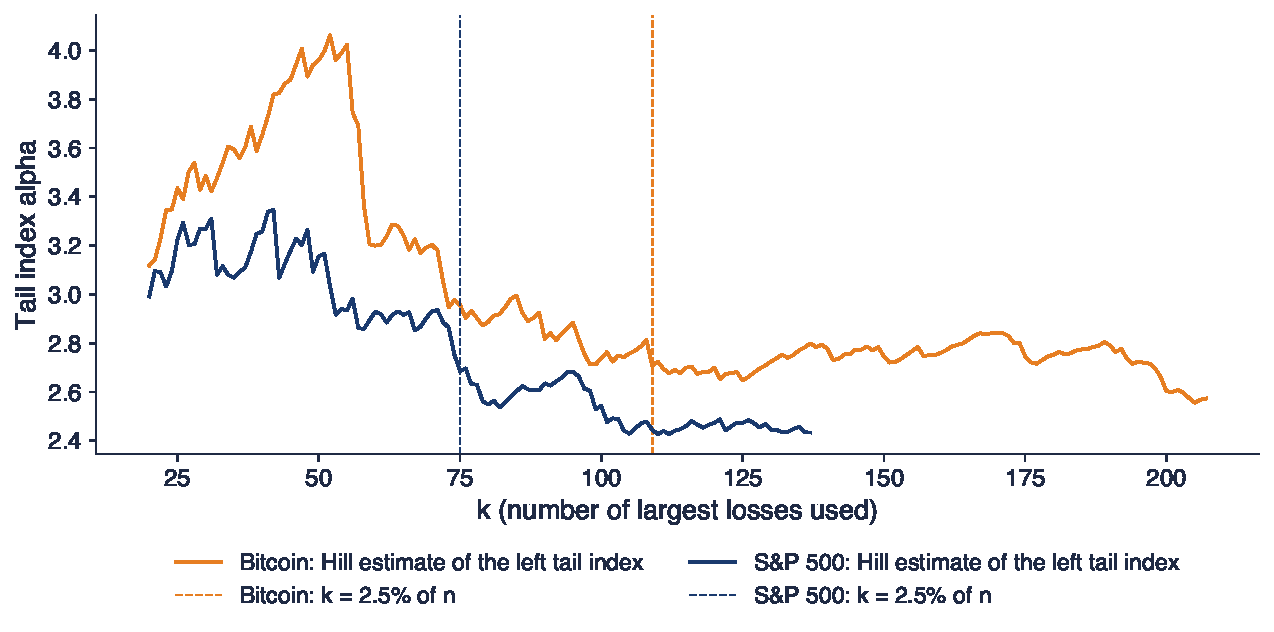
\includegraphics[width=0.96\textwidth,height=0.30\textheight,keepaspectratio]{ch14_sem_b1.pdf}
\end{center}
\vspace{-2mm}
\begin{center}
\scriptsize
\begin{tabular}{lrrrrrrrr}
\toprule
& $n$ & sd & skew. & exc.\ kurt. & vol.\ (actual $m$) & vol.\ (252) & $\hat\alpha$ left [95\% CI] & $\hat\alpha$ right \\
\midrule
Bitcoin & 4\,384 & $3.49$ & $-0.70$ & $12.0$ & $66.6$ & $55.3$ & $2.71$ $[2.20, 3.21]$ & $3.37$ \\
S\&P 500 & 3\,017 & $1.11$ & $-0.64$ & $15.8$ & $17.6$ & $17.6$ & $2.68$ $[2.08, 3.29]$ & $2.80$ \\
\bottomrule
\end{tabular}
\end{center}
\begin{itemize}
    \item Means: 0.118\% and 0.044\% a day; annual means 43.1\% ($m = 365.3$) and 11.2\% ($m = 251.4$); with 252 days Bitcoin's volatility would be 55.3\%
    \item Interpretation: no: the left-tail indices are almost equal and their intervals overlap; Bitcoin is about four times more volatile, but its tail has the same shape: the difference is in scale
\end{itemize}\sfmquantlet{Ch_14}{SFM_ch14_seminar}
\end{frame}

\begin{frame}{B2: Ethereum and Solana [Proposed]}
\itemsize{\footnotesize}
\begin{itemize}
\item \textbf{Question}: do the conclusions of B1 hold for two other large crypto assets? Model: B1.
\item \textbf{Inputs}: Ethereum since 2016, Solana since April 2020; daily log returns in \%
\item \textbf{Tasks}
\begin{enumerate}
    \item Compute the four moments of each series.
    \item Annualise the volatility with 365 and with 252 days.
    \item Compute both Hill indices with their 95\% intervals.
    \item Interpretation: which of the five assets of B1 and B2 has the heaviest left tail?
\end{enumerate}
\item \textbf{Report}: one table and two sentences
\item Notebook: section B2
\end{itemize}
\end{frame}

\ifsolutions
\begin{frame}{B2: Solution [Proposed]}
\itemsize{\footnotesize}
\begin{center}
\scriptsize
\begin{tabular}{lrrrrrrr}
\toprule
& $n$ & sd & skew. & exc.\ kurt. & vol.\ 365 & vol.\ 252 & $\hat\alpha$ left [95\% CI] \\
\midrule
Ethereum & 3\,913 & $4.99$ & $-0.20$ & $9.0$ & $95.3$ & $79.2$ & $2.62$ $[2.10, 3.15]$ \\
Solana & 2\,351 & $6.12$ & $-0.22$ & $7.9$ & $117.1$ & $97.2$ & $2.84$ $[2.11, 3.57]$ \\
\bottomrule
\end{tabular}
\end{center}
\begin{itemize}
    \item Right tails: $\hat\alpha = 3.09$ (Ethereum), $3.41$ (Solana): the left tail is heavier, as for Bitcoin
    \item Interpretation: Ethereum has the smallest point estimate ($2.62$), but all intervals overlap: with 58 to 97 tail observations we cannot rank the five tails; the volatilities differ clearly
\end{itemize}\sfmquantlet{Ch_14}{SFM_ch14_seminar}
\end{frame}
\fi

\begin{frame}{B3: Bitcoin and the S\&P 500 in Calm and Crisis [Solved]}
\itemsize{\footnotesize}
\begin{itemize}
\item \textbf{Question}: did the correlation between Bitcoin and equities change after 2020, and what happened in the 2020 and 2022 crises?
\item \textbf{Inputs}: Bitcoin and S\&P 500 closes since September 2014, joined on common days; daily and weekly (Friday to Friday) log returns
\item \textbf{Tasks}
\begin{enumerate}
    \item Compute the correlation before 2020 and from 2020 on, and test their equality with the Fisher $z$ test.
    \item Compute the correlation of daily and of weekly returns year by year and draw both.
    \item Compute the cumulative returns of both series in the COVID-19, Terra/Luna and FTX episodes.
    \item Compute Bitcoin's mean return on the worst 5\% of S\&P 500 days.
    \item Interpretation: does Bitcoin diversify an equity portfolio when it is most needed?
\end{enumerate}
\item \textbf{Report}: six numbers, the chart and two sentences
\item Notebook: section B3
\end{itemize}
\end{frame}

\begin{frame}{B3: Solution [Solved]}
\itemsize{\scriptsize}
\begin{center}
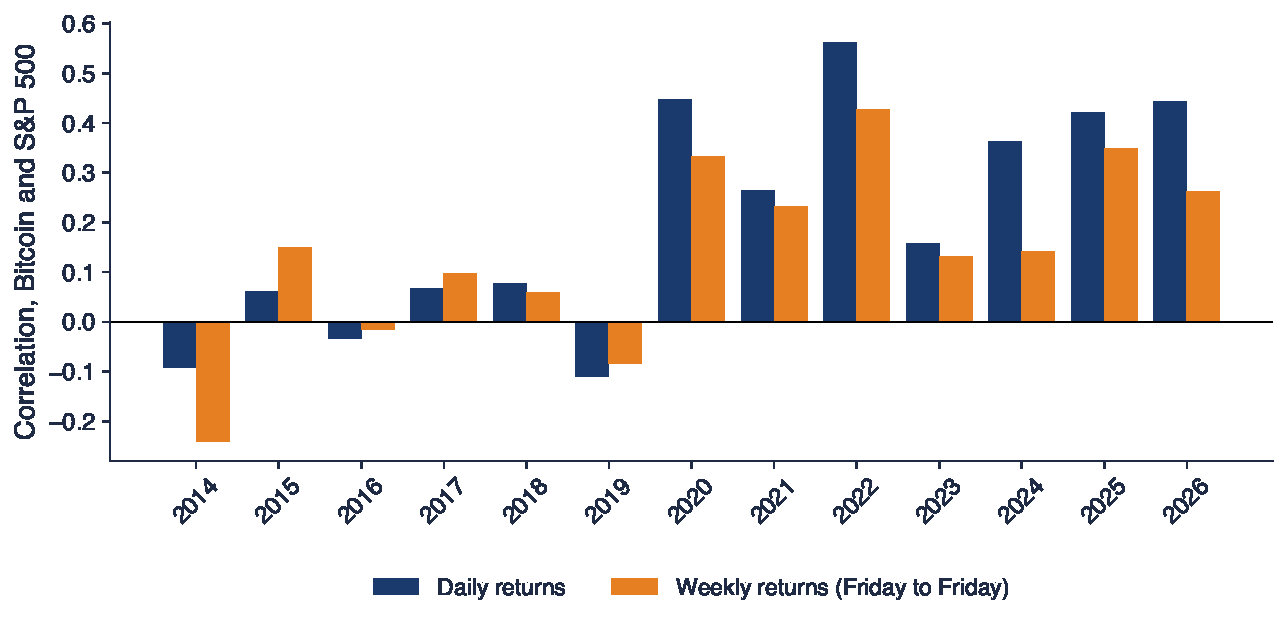
\includegraphics[width=0.96\textwidth,height=0.32\textheight,keepaspectratio]{ch14_sem_b3.pdf}
\end{center}
\vspace{-2mm}
\begin{itemize}
    \item Before 2020: $\hat\rho = 0.02$ ($n = 1\,330$); from 2020: $\hat\rho = 0.39$, 95\% CI $[0.35, 0.43]$ ($n = 1\,687$); Fisher $z = 10.71$, p $<$\,0.001
    \item Cumulative log returns (Bitcoin; S\&P 500): COVID-19 $-40.6\%$; $-41.4\%$; Terra/Luna $-23.0\%$; $-5.4\%$; FTX $-29.9\%$; $4.6\%$
    \item On the 151 worst S\&P 500 days (mean $-2.70\%$), Bitcoin returned on average $-2.77\%$; weekly correlation over the whole period 0.19, daily 0.24
    \item Interpretation: no: since 2020 the correlation is significantly positive, and on the worst equity days Bitcoin falls as much as the S\&P 500; crypto-specific crises (Terra, FTX) did not spread to equities
\end{itemize}\sfmquantlet{Ch_14}{SFM_ch14_seminar}
\end{frame}

\begin{frame}{B4: Bitcoin and Gold, Ethereum and the S\&P 500 [Proposed]}
\itemsize{\footnotesize}
\begin{itemize}
\item \textbf{Question}: is Bitcoin linked with gold, and does Ethereum behave like Bitcoin towards equities? Model: B3.
\item \textbf{Inputs}: Bitcoin and gold (XAU/USD) since 2014; Ethereum and S\&P 500 since 2016; prices joined on common days
\item \textbf{Tasks}
\begin{enumerate}
    \item Compute both correlations before and after 2020 and test their equality.
    \item Compute the correlations of 2022 and 2025, daily and weekly.
    \item Compute the mean return of Bitcoin on the worst 5\% of gold days, and of Ethereum on the worst 5\% of S\&P 500 days.
    \item Interpretation: is Bitcoin ``digital gold''?
\end{enumerate}
\item \textbf{Report}: one table and two sentences
\item Notebook: section B4
\end{itemize}
\end{frame}

\ifsolutions
\begin{frame}{B4: Solution [Proposed]}
\itemsize{\footnotesize}
\begin{center}
\scriptsize
\begin{tabular}{lrrrrrrr}
\toprule
& before 2020 & from 2020 & Fisher $z$ (p) & 2022 d./w. & 2025 d./w. & mean on bad days \\
\midrule
Bitcoin, gold & $-0.01$ & $0.15$ & $4.47$ ($<$\,0.001) & $0.15$/$0.11$ & $0.12$/$0.00$ & $-0.76$ \\
Ethereum, S\&P 500 & $0.02$ & $0.40$ & $10.23$ ($<$\,0.001) & $0.55$/$0.51$ & $0.46$/$0.33$ & $-4.42$ \\
\bottomrule
\end{tabular}
\end{center}
\begin{itemize}
    \item Bad days: the worst 5\% of days of the second series (gold; S\&P 500); mean of the first series in \%
    \item Interpretation: no: the correlation with gold rose only to 0.15 and Bitcoin does not hold value when gold falls or when stocks fall; Ethereum moves with equities even more than Bitcoin
\end{itemize}\sfmquantlet{Ch_14}{SFM_ch14_seminar}
\end{frame}
\fi

\begin{frame}{B5: How Stable Is USDC? [Solved]}
\itemsize{\footnotesize}
\begin{itemize}
\item \textbf{Question}: how far and for how long does USDC move away from 1 USD?
\item \textbf{Inputs}: USDC daily closes and lows since 1 January 2021
\item \textbf{Tasks}
\begin{enumerate}
    \item Compute the peg deviations in bp and their standard deviation and median absolute value.
    \item Compute the share of days in the classes below 1, 1--5, 5--10, 10--50 and above 50 bp, and draw them.
    \item Fit an AR(1) to the deviation and compute the half-life of a deviation.
    \item Compare the standard deviation before 2023 and after April 2023.
    \item Interpretation: can a treasurer treat USDC as cash?
\end{enumerate}
\item \textbf{Report}: six numbers, the chart and two sentences
\item Notebook: section B5
\end{itemize}
\end{frame}

\begin{frame}{B5: Solution [Solved]}
\itemsize{\scriptsize}
\begin{center}
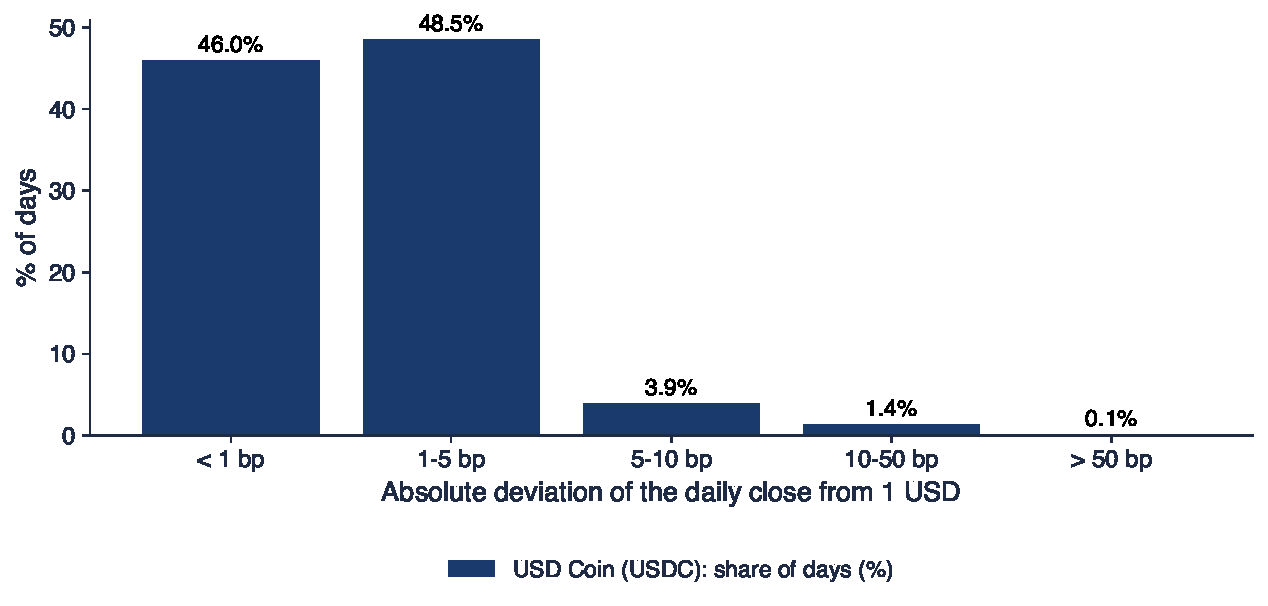
\includegraphics[width=0.96\textwidth,height=0.30\textheight,keepaspectratio]{ch14_sem_b5.pdf}
\end{center}
\vspace{-2mm}
\begin{itemize}
    \item $n = 2\,087$ days; sd 7.5 bp, median $|d_t|$ 1.1 bp; 1.5\% of days beyond 10 bp, 0.14\% beyond 50 bp; worst close $-285$ bp (11 March 2023), worst low $-1226$ bp
    \item AR(1): $\hat\phi = 0.290$ (se $0.021$), half-life 0.56 days; sd 5.8 bp in 2021--2022, 1.5 bp after April 2023
    \item Interpretation: almost always: on a typical day USDC is within a few bp and deviations close within a day; but the tail is real: on one weekend of 2023 a holder could lose 3\% at the close and 12\% at the low
\end{itemize}\sfmquantlet{Ch_14}{SFM_ch14_seminar}
\end{frame}

\begin{frame}{B6: USDT and DAI [Proposed]}
\itemsize{\footnotesize}
\begin{itemize}
\item \textbf{Question}: are USDT and DAI as stable as USDC? Model: B5.
\item \textbf{Inputs}: USDT and DAI daily closes and lows since 1 January 2021
\item \textbf{Tasks}
\begin{enumerate}
    \item Compute the standard deviation, the median absolute deviation and the shares beyond 10 and 50 bp.
    \item Find the worst close and the worst low of each coin, with their dates.
    \item Fit the AR(1) and compute the half-lives.
    \item Interpretation: which of the three coins keeps the peg best in normal times, and which in a crisis?
\end{enumerate}
\item \textbf{Report}: one table and two sentences
\item Notebook: section B6
\end{itemize}
\end{frame}

\ifsolutions
\begin{frame}{B6: Solution [Proposed]}
\itemsize{\footnotesize}
\begin{center}
\scriptsize
\begin{tabular}{lrrrrrrr}
\toprule
& sd & median $|d|$ & $>$10 bp (\%) & $>$50 bp (\%) & worst close & worst low & half-life \\
\midrule
USDT & $7.3$ & $3.1$ & $11.4$ & $0.14$ & $-41$ & $-515$ & $2.16$ \\
DAI & $10.8$ & $2.2$ & $10.7$ & $0.57$ & $-261$ & $-1030$ & $0.63$ \\
USDC & $7.5$ & $1.1$ & $1.5$ & $0.14$ & $-285$ & $-1226$ & $0.56$ \\
\bottomrule
\end{tabular}
\end{center}
\begin{itemize}
    \item Worst closes: USDT on 11 May 2022, DAI on 11 March 2023; deviations in bp, half-lives in days
    \item Interpretation: in normal times USDC is the tightest (median 1.1 bp) and USDT the loosest, with the slowest return to the peg; in March 2023 USDT stayed at the peg while USDC and DAI broke it: stability in calm times says little about crises
\end{itemize}\sfmquantlet{Ch_14}{SFM_ch14_seminar}
\end{frame}
\fi

\begin{frame}{B7: Risk of a Bitcoin Position [Solved]}
\itemsize{\footnotesize}
\begin{itemize}
\item \textbf{Question}: how much can a position of 100\,000 USD in Bitcoin lose in one day, and which model would have passed a backtest?
\item \textbf{Inputs}: Bitcoin closes since September 2014, daily log returns in \%
\item \textbf{Tasks}
\begin{enumerate}
    \item Compute VaR 1\% and ES 2.5\% by historical simulation, Normal, Student-t (maximum likelihood) and GARCH(1,1)-t for the next day.
    \item Convert them into USD with $W(1 - e^{-v/100})$.
    \item Backtest the one-day VaR 1\% since 2018: historical simulation on the last 365 days and GARCH(1,1)-t re-estimated every 365 days; count the exceptions and run the Kupiec test.
    \item Interpretation: which number would you report to a risk committee?
\end{enumerate}
\item \textbf{Report}: a table of eight numbers, the chart, two test results and two sentences
\item Notebook: section B7
\end{itemize}
\end{frame}

\begin{frame}{B7: Solution [Solved]}
\itemsize{\scriptsize}
\begin{center}
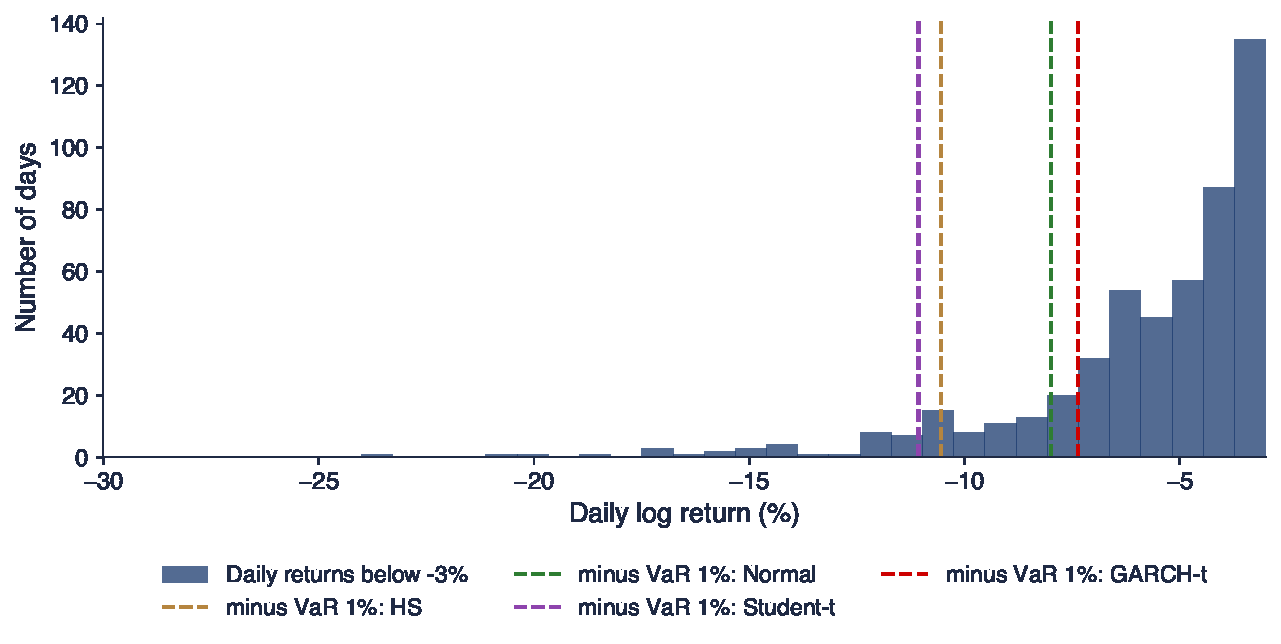
\includegraphics[width=0.96\textwidth,height=0.28\textheight,keepaspectratio]{ch14_sem_b7.pdf}
\end{center}
\vspace{-2mm}
\begin{center}
\scriptsize
\begin{tabular}{lrrrr}
\toprule
& HS & Normal & Student-t & GARCH-t \\
\midrule
VaR 1\% (\%) & $10.54$ & $7.99$ & $11.06$ & $7.37$ \\
VaR 1\% (USD) & 10\,006 & 7\,679 & 10\,474 & 7\,105 \\
ES 2.5\% (\%) & $10.84$ & $8.03$ & $13.37$ & $8.11$ \\
\bottomrule
\end{tabular}
\end{center}
\begin{itemize}
    \item $n = 4\,384$; Student-t $\hat\nu = 2.23$; GARCH-t $\hat\sigma_{t+1} = 2.83\%$, $\hat\nu = 3.18$; backtest since 1 January 2018 ($n = 3\,183$, expected 31.8): HS 29 exceptions, LR $= 0.26$ (p $= 0.61$); GARCH-t 41, LR $= 2.45$ (p $= 0.12$)
    \item Interpretation: report the historical VaR 1\% (10\,006 USD) as the long-run number and the GARCH-t VaR (7\,105 USD) as today's number; the Normal VaR is 24\% too low; both backtested models pass
\end{itemize}\sfmquantlet{Ch_14}{SFM_ch14_seminar}
\end{frame}

\begin{frame}{B8: Risk of an Ethereum Position [Proposed]}
\itemsize{\footnotesize}
\begin{itemize}
\item \textbf{Question}: does the conclusion of B7 hold for Ethereum? Model: B7.
\item \textbf{Inputs}: Ethereum closes since 2016; backtest since 1 January 2019
\item \textbf{Tasks}
\begin{enumerate}
    \item Compute VaR 1\% and ES 2.5\% by the four methods of B7, in \% and in USD.
    \item Backtest the two one-day VaR 1\% forecasts and run the Kupiec test.
    \item Find the largest number of exceptions in one calendar year for each model.
    \item Interpretation: which model would you keep for Ethereum?
\end{enumerate}
\item \textbf{Report}: one table and two sentences
\item Notebook: section B8
\end{itemize}
\end{frame}

\ifsolutions
\begin{frame}{B8: Solution [Proposed]}
\itemsize{\footnotesize}
\begin{center}
\scriptsize
\begin{tabular}{lrrrr}
\toprule
& HS & Normal & Student-t & GARCH-t \\
\midrule
VaR 1\% (\%) & $14.29$ & $11.40$ & $15.39$ & $10.95$ \\
VaR 1\% (USD) & 13\,312 & 10\,772 & 14\,263 & 10\,369 \\
ES 2.5\% (\%) & $14.77$ & $11.45$ & $18.13$ & $12.05$ \\
\bottomrule
\end{tabular}
\end{center}
\begin{itemize}
    \item Backtest since 1 January 2019 ($n = 2\,818$, expected 28.2): HS 30 exceptions (p $= 0.73$), at most 8 in one year; GARCH-t 22 (p $= 0.22$), at most 4 in one year
    \item Interpretation: both pass; HS is closer to the target rate, GARCH-t is slightly conservative but adapts faster; the Normal VaR is 20\% too low; keep HS for reporting and GARCH-t for daily limits
\end{itemize}\sfmquantlet{Ch_14}{SFM_ch14_seminar}
\end{frame}
\fi


%=============================================================================
\section{Part C: Open Questions and AI Critique}
%=============================================================================

\begin{frame}{C1: Did the Spot ETFs Change Bitcoin? [Proposed]}
\itemsize{\footnotesize}
\begin{itemize}
\item \textbf{Question}: since 11 January 2024 US investors can hold Bitcoin through spot ETFs traded on weekdays; did Bitcoin's volatility, its weekend pattern or its link with equities change?
\item \textbf{Inputs}: Bitcoin and S\&P 500; two years before and two years after the launch; models: B1, B3
\item \textbf{Tasks}
\begin{enumerate}
    \item Compute the annualised volatility in both windows and test the equality of variances (Brown--Forsythe).
    \item Compute the ratio of weekend to weekday variance in both windows.
    \item Compute the correlation with the S\&P 500 and the GARCH(1,1)-t persistence in both windows.
    \item Interpretation: can a before--after comparison prove an effect of the ETFs?
\end{enumerate}
\item \textbf{Report}: a table and a plan for a project
\item Notebook: section C1
\end{itemize}
\end{frame}

\ifsolutions
\begin{frame}{C1: Reference Analysis [Proposed]}
\itemsize{\footnotesize}
\begin{center}
\scriptsize
\begin{tabular}{lrr}
\toprule
Bitcoin & 11 Jan 2022 -- 10 Jan 2024 & 11 Jan 2024 -- 10 Jan 2026 \\
\midrule
annualised volatility (\%) & $55.2$ & $47.5$ \\
weekend/weekday variance & $0.30$ & $0.42$ \\
weekend share of squared returns (\%) & $10.8$ & $14.4$ \\
correlation with the S\&P 500 & $0.45$ & $0.37$ \\
GARCH(1,1)-t $\hat\alpha + \hat\beta$ & $1.000$ & $0.97$ \\
\bottomrule
\end{tabular}
\end{center}
\begin{itemize}
    \item Brown--Forsythe p $= 0.27$: the fall in volatility is not significant; the weekend share rose, the correlation fell
    \item No: rates, the April 2024 halving and the US election changed in the same window; a credible design uses a control group (coins without an ETF), intraday data around 9:30 New York time, or ETF flows as a continuous treatment
\end{itemize}\sfmquantlet{Ch_14}{SFM_ch14_seminar}
\end{frame}
\fi

\begin{frame}{C2: Audit an AI Answer [Proposed]}
\itemsize{\scriptsize}
\begin{itemize}
    \item A student asked an AI assistant to summarise the risks of Bitcoin and stablecoins. The answer:
    \item \aiprompt{(a) Bitcoin's annual volatility is 55.3\%: the daily standard deviation times sqrt(252).}
    \item \aiprompt{(b) The VaR 99\% of 100,000 USD in Bitcoin is -10\,543 USD.}
    \item \aiprompt{(c) On 11 March 2023 USDC lost 2.85 basis points.}
    \item \aiprompt{(d) TerraUSD was a fiat-backed stablecoin whose reserves were US Treasury bills.}
    \item \aiprompt{(e) Bitcoin is a safe haven: its correlation with the S\&P 500 is 0.02.}
    \item \aiprompt{(f) Bitcoin returns are less volatile at weekends than on weekdays.}
    \item Tasks
    \begin{itemize}
        \item 1. For each statement, say whether it is correct; if not, give the correct statement and, where possible, the correct number from the notebook (section C2).
        \item 2. Report: a list of six verdicts with one line of justification each.
    \end{itemize}
\end{itemize}
\end{frame}

\ifsolutions
\begin{frame}{C2: Solution [Proposed]}
\itemsize{\footnotesize}
\begin{itemize}
    \item (a) Wrong: crypto trades 365 days a year: $\sqrt{365}\,s = 66.6\%$
    \item (b) Wrong three times: the level is VaR 1\%, VaR is a positive loss, and a log-return VaR of 10.54\% is $100\,000(1 - e^{-10.54/100}) = 10\,006$ USD
    \item (c) Wrong unit: the close of 0.9715 is $-285$ bp, i.e.\ 2.85\%, not 2.85 bp
    \item (d) Wrong: UST was algorithmic, backed only by the LUNA token; that is why it could not be rescued
    \item (e) Wrong: 0.02 is the correlation before 2020; since 2020 it is 0.39, and on the worst 5\% of S\&P 500 days Bitcoin lost on average $-2.77\%$
    \item (f) Correct: the weekend variance is about a third to two thirds of the weekday variance (Lecture 14)
\end{itemize}\sfmquantlet{Ch_14}{SFM_ch14_seminar}
\end{frame}
\fi


%=============================================================================
\section{Wrap-Up}
%=============================================================================

\begin{frame}{What You Should Take from Today}
\itemsize{\small}
\begin{itemize}
    \item Annualise crypto with 365 days; never mix 252 and 365 in one ratio
    \item A fall of $d$ needs a gain of $d/(1 - d)$; crypto drawdowns of 75--85\% need gains of 300--570\%
    \item Peg deviations are measured in basis points; they are tiny in normal times and large in a run
    \item Since 2020 Bitcoin moves with equities; it is not a safe haven in this sample
    \item An AI answer is a draft: check the annualisation, the VaR level and sign, and the units
\end{itemize}
\end{frame}

\begin{frame}{After the Seminar}
\itemsize{\small}
\begin{itemize}
    \item Lecture 14 develops each topic of today: blockchain basics, crypto as an asset class, efficiency, correlation, bubbles, ETFs, stablecoins and regulation
    \item Try the [Proposed] tasks in the notebook; the solutions are discussed in class
    \item C1 can grow into a team project: a control group, intraday data, ETF flows
    \item Reading: \refFHH, Ch.~23; \refLT; \refLVN
\end{itemize}
\end{frame}


%=============================================================================
\section{References}
%=============================================================================

\begin{frame}{References}
\itemsize{\tiny}
\begin{itemize}
    \item Baur, D.G., Lucey, B.M. (2010). \href{https://doi.org/10.1111/j.1540-6288.2010.00244.x}{Is gold a hedge or a safe haven? An analysis of stocks, bonds and gold}. \textit{Financial Review}, 45(2), 217--229.
    \item Franke, J., Härdle, W.K., Hafner, C.M. (2019). \href{https://doi.org/10.1007/978-3-030-13751-9}{\textit{Statistics of Financial Markets: An Introduction}}, 5th ed. Springer.
    \item Griffin, J.M., Shams, A. (2020). \href{https://doi.org/10.1111/jofi.12903}{Is Bitcoin really untethered?} \textit{Journal of Finance}, 75(4), 1913--1964.
    \item Hill, B.M. (1975). \href{https://doi.org/10.1214/aos/1176343247}{A simple general approach to inference about the tail of a distribution}. \textit{Annals of Statistics}, 3(5), 1163--1174.
    \item Kupiec, P.H. (1995). \href{https://doi.org/10.3905/jod.1995.407942}{Techniques for verifying the accuracy of risk measurement models}. \textit{Journal of Derivatives}, 3(2), 73--84.
    \item Liu, J., Makarov, I., Schoar, A. (2023). \href{https://doi.org/10.3386/w31160}{Anatomy of a run: the Terra Luna crash}. NBER Working Paper 31160.
    \item Liu, Y., Tsyvinski, A. (2021). \href{https://doi.org/10.1093/rfs/hhaa113}{Risks and returns of cryptocurrency}. \textit{Review of Financial Studies}, 34(6), 2689--2727.
    \item Lyons, R.K., Viswanath-Natraj, G. (2023). \href{https://doi.org/10.1016/j.jimonfin.2022.102777}{What keeps stablecoins stable?} \textit{Journal of International Money and Finance}, 131, 102777.
    \item SEC, U.S. Securities and Exchange Commission (2024). \href{https://www.sec.gov/newsroom/speeches-statements/gensler-statement-spot-bitcoin-011023}{Statement on the approval of spot Bitcoin exchange-traded products}, 10 January 2024.
    \item Treasury, Federal Reserve and FDIC (2023). \href{https://www.federalreserve.gov/newsevents/pressreleases/monetary20230312b.htm}{Joint statement by the Department of the Treasury, Federal Reserve, and FDIC}, 12 March 2023.
\end{itemize}
\end{frame}

\end{document}
